\documentclass[11pt,a4paper]{article}
\usepackage[margin=2.2cm]{geometry}
\usepackage{amsmath,amssymb}
\usepackage{booktabs,array}
\usepackage{graphicx}
\usepackage{subcaption}
\usepackage{enumitem}
\usepackage{pifont}
\usepackage{rotating}
\usepackage[hidelinks]{hyperref}
\graphicspath{{../results/}}
\setlist{itemsep=2pt,topsep=4pt}

\title{Heuristic-guided reinforcement learning\\on toy combinatorial problems}
\author{Luis Felipe Cattelan}
\date{\today}

\begin{document}
\maketitle

\begin{abstract}
We compare ways of using a heuristic policy to help reinforcement learning, on four toy problems with known
heuristics and six guide heuristics in total, one of them evolved by an LLM (EoH) for a related bin-packing task.
The 21 main methods cover offline warm starts (behaviour cloning, DAgger, IQL, HUBL, HuRL), use of the heuristic during
PPO (kickstarting, a constant anchor, a residual policy, Jump-Start RL, HEPO), off-policy learning that keeps the
heuristic's data (DQfD, IQL offline $\to$ online) and a model-based teacher: the heuristic improved by Monte-Carlo
rollouts and distilled with DAgger. Follow-up experiments add a colleague's Crafter methods, fading and self-ending
versions of the pull towards the heuristic, and our methods run on Crafter. Every method gets 10 seeds and 1.5M
environment steps (on Crafter 3 seeds and 1M steps). We ask whether a method (1)~ends better than PPO from scratch, (2)~passes the heuristic sooner and
(3)~ends better than the heuristic. The main finding is that the regime decides: a lasting pull towards the heuristic
pays only until RL alone would pass the heuristic, so it is the best method on Crafter (where PPO stays far below the
heuristic) and among the worst on our problems (where PPO passes it). Where RL can pass the heuristic,
\emph{Rollout-DAgger $\to$ PPO + KL} is the most reliable (best mean rank, never worse than PPO from scratch, at the
cost of 80--500M simulated steps); without a simulator, IQL (+ HUBL) $\to$ PPO + KL and imitation that ends when the
policy matches the heuristic. Online IQL, which never left the heuristic, does so once its advantage weights are
normalised; it is then the best method on knapsack and inventory, and with a discount of 0.99 the second-best method
overall (best with Sum of Squares and on load balancing, but failing on knapsack).
\end{abstract}

\section{Setting}

\paragraph{Questions.} Given a decent heuristic policy $\pi_H$ for a sequential decision problem, which ways of
feeding it into reinforcement learning
\begin{enumerate}[label=\textbf{Q\arabic*}, leftmargin=*]
\item end \textbf{better than RL from scratch} (final metric of the trained policy, same environment budget)?
\item \textbf{reach the heuristic's level faster} than RL from scratch (environment steps until the policy first
  beats the heuristic, counting the heuristic's demonstration steps)?
\item end \textbf{better than the heuristic} itself?
\end{enumerate}

\paragraph{Problems.} Four problems with fixed-length episodes, a discrete (masked) action space, a small vector
observation and a per-episode metric where lower is better (Table~\ref{tab:problems}). Each has a \emph{guide}
heuristic that the methods learn from and, where we know one, a stronger \emph{reference} heuristic that shows how
much room there is above the guide. Bin packing is run with three guides: the weak Best Fit, the near-optimal Sum of
Squares, and an LLM-evolved heuristic (below), giving six experiments.

\begin{table}[h]
\centering\small
\setlength{\tabcolsep}{4pt}
\newcolumntype{L}[1]{>{\raggedright\arraybackslash}p{#1}}
\begin{tabular}{L{2.3cm}L{5.0cm}L{2.3cm}L{2.9cm}L{2.3cm}}
\toprule
Problem & Decision (episode) & Metric & Guides & Reference \\
\midrule
Online bin packing & place an item of size 3 or 4 ($p = 2/3, 1/3$) into a bin of capacity 12 (200 items)
  & wasted capacity & Best Fit 9.68\%, Sum of Squares 2.36\%, EoH-evolved 11.48\% & Sum of Squares 2.36\% \\
Online knapsack & accept/reject items, weight and value uniform on $\{1..10\}$, capacity 250 (200 items)
  & gap to the offline fractional optimum & static density threshold 3.69\% & adaptive threshold 1.24\% \\
Load balancing & send a job (size $\sim$Exp(1)) to one of 4 FIFO servers with speeds 0.4--1.6, load 0.85 (200 jobs)
  & mean sojourn time & shortest expected delay 1.73 & --- (least work left: 1.96) \\
Lost-sales inventory & order 0--15 units, lead time 3, Poisson(5) demand, holding 1, lost sale 9 (100 periods)
  & mean cost per period & base stock ($S = 23$) 6.94 & capped base stock 6.70 \\
\bottomrule
\end{tabular}
\caption{The toy problems. Heuristic values are on 256 fixed evaluation episodes. A uniformly random policy scores
13.6\%, 55.0\%, 3.99 and 129.0 respectively.}
\label{tab:problems}
\end{table}

\paragraph{The EoH-evolved heuristic.} The third bin-packing guide is the best heuristic of twelve EoH searches in the
companion project RL-AHD-OBP (\texttt{w10\_on\_half4}, search fitness 0.00537), evolved by an LLM for online bin
packing with Weibull items and capacity 100. It is a score function $\mathrm{score}(\mathit{item}, \mathit{bins},
\mathit{progress}, \mathit{history\_mean}, \mathit{history\_std})$: tightness $1/(\mathit{bins} - \mathit{item})$,
minus a penalty for bins left loose relative to the typical item, plus a progress-dependent bonus near the tightest
fit. It is copied verbatim (\texttt{problems/binpack.py}) and called exactly as EoH's evaluator calls it: the bin
array holds one entry per opened feasible bin \emph{plus the pool of untouched bins at capacity}, and the item history
excludes the current item. A test checks that it packs the same number of bins as EoH's own loop on every episode,
and a vectorised version picks the same action as the verbatim function in all 51,200 tested states. Tuned for a
different item distribution, it is a weak guide here: 11.48\% waste, worse than Best Fit (9.68\%).

\section{Methods}

All methods share one PPO: separate 2$\times$128 tanh MLPs for actor and critic, 16 parallel environments
$\times$ 128 steps per update, 4 epochs, minibatch 512, Adam $3\cdot10^{-4}$, $\gamma = 1$ (finite horizon), GAE
$\lambda = 0.95$, clip 0.2, entropy 0.01, value coefficient 0.5, gradient norm 0.5. Infeasible actions are masked
(logit $-10^9$). Method-specific hyperparameters were set once from the papers or the companion projects and not
tuned, except where a stated failure forced a change (online IQL, rollout labels). Table~\ref{tab:methods} lists how
each method uses the heuristic. Section~\ref{sec:followup} adds 19 variants (the Crafter study's methods,
fading and self-ending pulls, rollout labels without the significance test, online IQL with normalised advantage
weights); they are in all the result tables.

\begin{table}[h]
\centering\small
\setlength{\tabcolsep}{4pt}
\newcolumntype{L}[1]{>{\raggedright\arraybackslash}p{#1}}
\begin{tabular}{L{4.2cm}L{8.3cm}L{3.2cm}}
\toprule
Heuristic used & Methods & Heuristic needed \\
\midrule
not at all & PPO from scratch & --- \\
offline, before RL (fixed dataset) & BC, IQL, IQL + HUBL warm starts; HuRL's $h(s)$ & 64 episodes \\
interactively, before RL & DAgger; Rollout-DAgger (also needs a simulator) & 64 episodes of labels \\
online, during RL & kickstarting, anchor, Jump-Start RL, HEPO, DQfD, IQL offline $\to$ online & every step \\
inside the deployed policy & residual policy & every step, also at test time \\
\bottomrule
\end{tabular}
\caption{How the methods use the heuristic.}
\label{tab:methods}
\end{table}

\subsection{Offline warm starts}
\begin{enumerate}[leftmargin=*]
\item \textbf{PPO from scratch.} The heuristic is not used.
\item \textbf{BC $\to$ PPO (naive).} The heuristic plays 64 episodes (12,800 steps; 6,400 for inventory); the actor is
  trained by cross-entropy on its actions (hard labels, masked softmax, Adam $10^{-3}$, minibatch 512, 10 epochs).
  The critic stays random. PPO then starts from the cloned actor.
\item \textbf{BC $\to$ PPO + KL.} Same, but PPO adds $\beta_u\,\mathrm{KL}(\pi \,\|\, \pi_{\mathrm{BC}})$ to the
  frozen clone, with $\beta$ decaying linearly from 1 to 0 by 50\% (or 20\%) of training, and the first 10 updates
  train only the critic.
\item \textbf{DAgger $\to$ PPO (naive / + KL).} The same 64-episode budget in 4 rounds: round 0 is the heuristic's
  own play, later rounds let the current policy act (greedily) while the heuristic labels the visited states; retrain
  on the aggregate after each round. Then PPO as in 2 or 3.
\item \textbf{HuRL} (Cheng et al., 2021). A heuristic value $h(s)$ is fitted by least squares to the heuristic's
  Monte-Carlo returns on the demonstrations. PPO then trains on the reshaped problem
  $\tilde r = r + (1-\lambda_n)\gamma\, h(s')$, $\tilde\gamma = \lambda_n\gamma$, with
  $\lambda_n = \lambda_0 + (1-\lambda_0)\tanh(\omega n)$, $\lambda_0 = 0.9$, reaching $\approx 1$ at half of
  training. Run from scratch and from the BC policy (\textbf{BC $\to$ HuRL}).
\item \textbf{IQL $\to$ PPO + KL.} Offline RL on 64 heuristic episodes in which episode $i$ takes a uniformly random
  feasible action with probability $\varepsilon_i \in [0, 0.5]$ (mixed quality, wider state coverage). Discrete IQL
  (Kostrikov et al., 2022): $V$ by expectile regression ($\tau = 0.7$) on $Q_{\mathrm{target}}(s, a)$ of data
  actions, $Q$ by regression on $r + \gamma V(s')$ with $\gamma = 0.99$, and an advantage-weighted actor
  $\max \exp(\beta (Q - V)) \log \pi(a|s)$, $\beta = 10$, weights capped at 100; 10k updates. Only the actor is passed
  on; PPO + KL as in 3.
\item \textbf{IQL + HUBL $\to$ PPO + KL} (Geng et al., 2023). Same, with HUBL's relabelled targets
  $\tilde r = r + \gamma\lambda h'$, $\tilde\gamma = \gamma(1-\lambda)$, $h$ the Monte-Carlo return-to-go and
  $\lambda = 0.1\cdot\mathrm{rank}(\tau)/n$ per trajectory.
\end{enumerate}
BC and IQL both learn offline from a fixed dataset; the difference is that BC copies the heuristic's actions and ignores
rewards, so at best it equals the heuristic, while IQL weights the actions in its data by their estimated advantage
and can improve on them within the data's support.

\subsection{Using the heuristic during RL}
For these methods every observation is extended by a one-hot of the heuristic's action in that state
(\texttt{hgrl/online.py}). Except for the residual policy, the networks never see it: it is only the target of the
anchor, so the trained policy runs without the heuristic.
\begin{enumerate}[leftmargin=*,resume]
\item \textbf{Kickstarting} (Schmitt et al., 2018). PPO from scratch plus $c_u \cdot$ cross-entropy to the heuristic's
  action on every state PPO visits, $c$ decaying linearly from 1 to 0 by 50\% of training.
\item \textbf{BC $\to$ PPO + heuristic anchor.} The recipe that beat its teacher in RL-AHD-OBP: BC warm start,
  10 critic-only updates, then PPO plus a constant $0.1 \cdot$ cross-entropy to the heuristic's action on the visited
  states (anchored to the heuristic, not to the clone). Also with a \textbf{4$\times$ batch} (64 environments per
  update), which was what unlocked beating the teacher there; and after \textbf{IQL + HUBL} instead of BC.
\item \textbf{Residual policy on the heuristic} (Silver et al., 2018). $\pi(a|s) \propto
  \exp(f_\theta(s, a_H)_a + \kappa\, \mathbf 1[a = a_H])$ with $\kappa = 3$: the network $f$ (which also sees $a_H$)
  starts at zero, so training starts at a softened heuristic and learns where to depart from it. PPO trains the
  combined policy; 10 critic-only updates first. The deployed policy needs the heuristic.
\item \textbf{Jump-Start RL} (Uchendu et al., 2023). The heuristic plays the first $h$ steps of every episode and the
  policy the rest; $h$ decreases linearly from the full episode to 0 by 50\% of training. Only the policy's steps
  enter the loss.
\item \textbf{HEPO} (Lee et al., 2024). Maximise $(1+\alpha)J(\pi) + H(\pi)$ subject to $J(\pi) \ge J(\pi_H)$.
  Adaptation: the heuristic reward is $h(s,a) = 0.1\cdot\mathbf 1[a = \pi_H(s)]$, whose optimal policy is the
  heuristic itself, so $\pi_H$ is the heuristic (not trained). Half of the environments are played by $\pi_H$ on the
  same random sequences; $\pi$ is updated on both halves with advantage $(1+\alpha)A_r + A_h$ and
  $\pi_H(a\mid s) = 1$ in the importance ratio; $\alpha \leftarrow \max(0, \alpha - (\hat J(\pi) - \hat J(\pi_H)))$
  from Monte-Carlo returns.
\end{enumerate}

\subsection{A model-based teacher: rollout improvement of the heuristic}
\begin{enumerate}[leftmargin=*,resume]
\item \textbf{Rollout-DAgger $\to$ PPO + KL} (rollout: Bertsekas, 1997; Tesauro \& Galperin, 1996; distillation as in
  Expert Iteration, Anthony et al., 2017). In a state $s$, every feasible action $a$ is tried and the heuristic
  finishes the episode on $M = 32$ freshly drawn futures (items, demand, arrivals not yet revealed), the same draws
  for every action. That is one step of policy iteration on the heuristic, never worse than it in expectation. With
  few samples, however, the argmax mostly picks noise, and the small losses add up over an episode (Sum of Squares:
  2.2\% $\to$ 5.2\% waste with 16 samples). So an action replaces the heuristic's only if its paired gain over the
  heuristic action is two standard errors above zero. These labels replace the heuristic's in DAgger (same 4 rounds
  of 16 episodes); then PPO + KL as in 3. Also with the KL to the clone \textbf{held} at 0.1
  (\textbf{Rollout-DAgger $\to$ PPO + held KL}). It needs a simulator that can copy its state and redraw the
  unrevealed future, and spends 80--500M simulated steps per run on labels (Table~\ref{tab:rollout}), which are not
  counted in the 1.5M environment steps.
\end{enumerate}

\subsection{Off-policy RL that keeps the heuristic's data}
\begin{enumerate}[leftmargin=*,resume]
\item \textbf{DQfD} (Hester et al., 2018). Double DQN on 64 pure heuristic episodes, pretrained for 10k updates, then
  online with $\varepsilon$-greedy exploration ($0.1 \to 0.01$ over half of training). Every update adds a
  large-margin loss $\max_a [Q(s,a) + 0.1\cdot\mathbf 1[a \neq a_H]] - Q(s, a_H)$ on the heuristic's samples. Half of
  each batch of 512 comes from the heuristic's data, half from the agent's replay buffer (symmetric sampling, Ball
  et al., 2023); one update per vector step; $\gamma = 1$.
\item \textbf{IQL offline $\to$ online} (Kostrikov et al., 2022). IQL on the same mixed data as method 6, then
  continued online, critic included, with the same symmetric sampling. Two changes were needed: $\gamma = 1$, and
  $\beta = 3$: with $\beta = 10$ the weights $\exp(\beta A)$ on the noisy advantages of fresh online data collapsed the
  actor on knapsack (gap 4\% $\to$ 40\%).
\end{enumerate}

\paragraph{Protocol.} 10 seeds per method and experiment, 1.5M environment steps. Offline data and DAgger episodes
(12,800 steps; 6,400 for inventory) are counted as environment interaction; HEPO's heuristic half is part of its PPO
steps; the simulated steps of Rollout-DAgger are not counted. Policies are evaluated greedily every 20,480 steps on 64
fixed episodes (learning curves) and at the end on 256 fixed episodes, the same for every method and heuristic. Q1 and
Q3 use a one-sided Welch $t$-test at 5\%; Q2 compares median steps. All runs were made on one machine: PPO on bin
packing is chaotic enough that floating-point differences between machines lead to different policies (a run of
PPO from scratch ended at 4.12\% waste on one machine and 6.05\% on another), so results from different machines
are not comparable run by run.

\section{Results}

% generated by report/make_tables.py -- do not edit by hand
\begin{table}[t]
\centering
\footnotesize
\setlength{\tabcolsep}{2.6pt}
\begin{tabular}{lcccccccc}
\toprule
Method & \shortstack{Bin packing\\(Best Fit)} & \shortstack{Bin packing\\(Sum of Sq.)} & \shortstack{Knapsack\\(static thr.)} & \shortstack{Load bal.\\(SED)} & \shortstack{Inventory\\(base stock)} & Q1 & Q2 & Q3 \\
\midrule
PPO from scratch & -- -- \ding{51} & -- -- $\approx$ & -- -- \ding{51} & -- -- \ding{51} & -- -- \ding{51} & -- & -- & 4/5 \\
BC $\to$ PPO (naive) & $\approx$ \ding{55} \ding{51} & $\approx$ \ding{51} \ding{51} & $\approx$ \ding{51} \ding{51} & $\approx$ \ding{51} \ding{51} & $\approx$ \ding{51} \ding{51} & 0/5 & 4/5 & 5/5 \\
BC $\to$ PPO + KL (50\%) & $\approx$ \ding{55} \ding{51} & $\approx$ \ding{51} \ding{51} & \ding{55} \ding{51} \ding{51} & \ding{55} \ding{51} \ding{51} & \ding{55} \ding{51} \ding{51} & 0/5 & 4/5 & 5/5 \\
BC $\to$ PPO + KL (20\%) & $\approx$ \ding{55} \ding{51} & $\approx$ \ding{51} \ding{51} & \ding{55} \ding{51} \ding{51} & $\approx$ \ding{51} \ding{51} & $\approx$ \ding{51} \ding{51} & 0/5 & 4/5 & 5/5 \\
DAgger $\to$ PPO (naive) & $\approx$ \ding{51} \ding{51} & $\approx$ \ding{51} \ding{51} & \ding{55} \ding{51} \ding{51} & \ding{55} \ding{51} \ding{51} & $\approx$ \ding{51} \ding{51} & 0/5 & 5/5 & 5/5 \\
DAgger $\to$ PPO + KL (50\%) & $\approx$ \ding{55} \ding{51} & $\approx$ \ding{51} \ding{51} & \ding{55} \ding{55} \ding{51} & \ding{55} \ding{51} \ding{51} & $\approx$ \ding{51} \ding{51} & 0/5 & 3/5 & 5/5 \\
HuRL (from scratch) & $\approx$ \ding{51} \ding{51} & $\approx$ \ding{55} $\approx$ & \ding{55} \ding{51} \ding{51} & \ding{51} \ding{55} \ding{51} & $\approx$ \ding{55} \ding{51} & 1/5 & 2/5 & 4/5 \\
BC $\to$ HuRL & $\approx$ \ding{51} \ding{51} & $\approx$ \ding{51} \ding{51} & \ding{55} \ding{51} \ding{51} & $\approx$ \ding{51} \ding{51} & $\approx$ \ding{51} \ding{51} & 0/5 & 5/5 & 5/5 \\
HEPO (from scratch) & \ding{55} \ding{51} $\approx$ & $\approx$ \ding{51} $\approx$ & \ding{55} \ding{51} \ding{51} & \ding{55} \ding{51} \ding{51} & \ding{55} \ding{55} \ding{51} & 0/5 & 4/5 & 3/5 \\
IQL $\to$ PPO + KL & $\approx$ \ding{51} \ding{51} & \ding{51} \ding{51} \ding{51} & $\approx$ \ding{51} \ding{51} & \ding{55} \ding{51} \ding{51} & $\approx$ \ding{51} \ding{51} & 1/5 & 5/5 & 5/5 \\
IQL + HUBL $\to$ PPO + KL & $\approx$ \ding{51} \ding{51} & $\approx$ \ding{51} \ding{51} & $\approx$ \ding{51} \ding{51} & \ding{55} \ding{51} \ding{51} & \ding{55} \ding{51} \ding{51} & 0/5 & 5/5 & 5/5 \\
\bottomrule
\end{tabular}
\caption{Scorecard for the three questions. Each cell gives Q1 Q2 Q3 for one experiment: Q1 final metric better than PPO from scratch, Q2 beats the guide heuristic in fewer environment steps than PPO from scratch, Q3 final metric better than the guide heuristic. \ding{51}~yes, \ding{55}~no (significantly worse, slower or never), $\approx$~no significant difference. Q1 and Q3 use a one-sided Welch $t$-test at 5\% over the 5 seeds (Q3 against the heuristic's value); Q2 compares the median steps of Table~\ref{tab:beat}. Last columns: number of experiments with \ding{51}.}
\label{tab:scorecard}
\end{table}

\begin{table}[t]
\centering
\small
\setlength{\tabcolsep}{4pt}
\begin{tabular}{lrrrrr}
\toprule
Method & \shortstack{Bin packing\\(Best Fit)} & \shortstack{Bin packing\\(Sum of Sq.)} & \shortstack{Knapsack\\(static thr.)} & \shortstack{Load bal.\\(SED)} & \shortstack{Inventory\\(base stock)} \\
\midrule
\textit{Guide heuristic} & 9.68 & 2.36 & 3.69 & 1.73 & 6.94 \\
\midrule
PPO from scratch & 2.48\,{\scriptsize$\pm$0.85} & 2.48\,{\scriptsize$\pm$0.85} & 1.45\,{\scriptsize$\pm$0.09} & 1.64\,{\scriptsize$\pm$0.02} & 6.70\,{\scriptsize$\pm$0.02} \\
BC $\to$ PPO (naive) & 3.62\,{\scriptsize$\pm$1.48} & 1.95\,{\scriptsize$\pm$0.28} & 1.64\,{\scriptsize$\pm$0.25} & 1.66\,{\scriptsize$\pm$0.02} & 6.70\,{\scriptsize$\pm$0.02} \\
BC $\to$ PPO + KL (50\%) & \textbf{1.63\,{\scriptsize$\pm$0.23}} & 1.75\,{\scriptsize$\pm$0.16} & 1.56\,{\scriptsize$\pm$0.06} & 1.67\,{\scriptsize$\pm$0.02} & 6.72\,{\scriptsize$\pm$0.02} \\
BC $\to$ PPO + KL (20\%) & 2.63\,{\scriptsize$\pm$1.11} & 1.78\,{\scriptsize$\pm$0.08} & 1.70\,{\scriptsize$\pm$0.19} & 1.67\,{\scriptsize$\pm$0.02} & 6.73\,{\scriptsize$\pm$0.04} \\
DAgger $\to$ PPO (naive) & 2.22\,{\scriptsize$\pm$0.98} & 1.94\,{\scriptsize$\pm$0.14} & 1.82\,{\scriptsize$\pm$0.16} & 1.67\,{\scriptsize$\pm$0.01} & \textbf{6.68\,{\scriptsize$\pm$0.01}} \\
DAgger $\to$ PPO + KL (50\%) & 3.67\,{\scriptsize$\pm$1.97} & 1.68\,{\scriptsize$\pm$0.09} & 1.77\,{\scriptsize$\pm$0.15} & 1.69\,{\scriptsize$\pm$0.02} & 6.68\,{\scriptsize$\pm$0.03} \\
HuRL (from scratch) & 1.66\,{\scriptsize$\pm$0.31} & 1.99\,{\scriptsize$\pm$0.38} & 1.74\,{\scriptsize$\pm$0.21} & \textbf{1.62\,{\scriptsize$\pm$0.01}} & 6.71\,{\scriptsize$\pm$0.02} \\
BC $\to$ HuRL & 1.70\,{\scriptsize$\pm$0.31} & 2.07\,{\scriptsize$\pm$0.13} & 1.63\,{\scriptsize$\pm$0.14} & 1.65\,{\scriptsize$\pm$0.02} & 6.71\,{\scriptsize$\pm$0.03} \\
HEPO (from scratch) & 9.68\,{\scriptsize$\pm$0.00} & 2.40\,{\scriptsize$\pm$0.05} & 3.05\,{\scriptsize$\pm$0.21} & 1.72\,{\scriptsize$\pm$0.00} & 6.75\,{\scriptsize$\pm$0.03} \\
IQL $\to$ PPO + KL & 2.02\,{\scriptsize$\pm$0.60} & \textbf{1.51\,{\scriptsize$\pm$0.27}} & 1.55\,{\scriptsize$\pm$0.15} & 1.68\,{\scriptsize$\pm$0.01} & 6.70\,{\scriptsize$\pm$0.03} \\
IQL + HUBL $\to$ PPO + KL & 2.00\,{\scriptsize$\pm$0.18} & 1.61\,{\scriptsize$\pm$0.13} & \textbf{1.44\,{\scriptsize$\pm$0.10}} & 1.68\,{\scriptsize$\pm$0.01} & 6.74\,{\scriptsize$\pm$0.03} \\
\bottomrule
\end{tabular}
\caption{Final performance of the trained policy (greedy, 256 fixed evaluation episodes; mean $\pm$ std over 5 seeds; best per column in bold). Bin packing: wasted capacity (\%); knapsack: gap to the offline optimum (\%); load balancing: mean sojourn time; inventory: mean cost per period. Lower is better everywhere.}
\label{tab:final}
\end{table}

\begin{table}[t]
\centering
\small
\setlength{\tabcolsep}{4pt}
\begin{tabular}{lrrrrr}
\toprule
Method & \shortstack{Bin packing\\(Best Fit)} & \shortstack{Bin packing\\(Sum of Sq.)} & \shortstack{Knapsack\\(static thr.)} & \shortstack{Load bal.\\(SED)} & \shortstack{Inventory\\(base stock)} \\
\midrule
PPO from scratch & 573k & 1157k & 225k & 205k & 102k \\
BC $\to$ PPO (naive) & 812k & 33k & 136k & \textbf{13k} & \textbf{6k} \\
BC $\to$ PPO + KL (50\%) & 771k & 54k & 115k & \textbf{13k} & \textbf{6k} \\
BC $\to$ PPO + KL (20\%) & 648k & 74k & 115k & \textbf{13k} & \textbf{6k} \\
DAgger $\to$ PPO (naive) & 443k & 54k & 177k & \textbf{13k} & \textbf{6k} \\
DAgger $\to$ PPO + KL (50\%) & 832k & 279k & 484k & \textbf{13k} & \textbf{6k} \\
HuRL (from scratch) & \textbf{156k} & 1221k & 115k & 504k & 191k \\
BC $\to$ HuRL & 218k & 730k & 115k & \textbf{13k} & \textbf{6k} \\
HEPO (from scratch) & 328k & 41k & 123k & 143k & 164k \\
IQL $\to$ PPO + KL & 566k & \textbf{13k} & 115k & \textbf{13k} & \textbf{6k} \\
IQL + HUBL $\to$ PPO + KL & 545k & 54k & \textbf{13k} & \textbf{13k} & \textbf{6k} \\
\bottomrule
\end{tabular}
\caption{Environment steps until the policy first beats its guide heuristic on the 64 evaluation episodes of the learning curves (median over seeds; includes the heuristic's demonstration steps).}
\label{tab:beat}
\end{table}


\begin{sidewaysfigure}
\centering
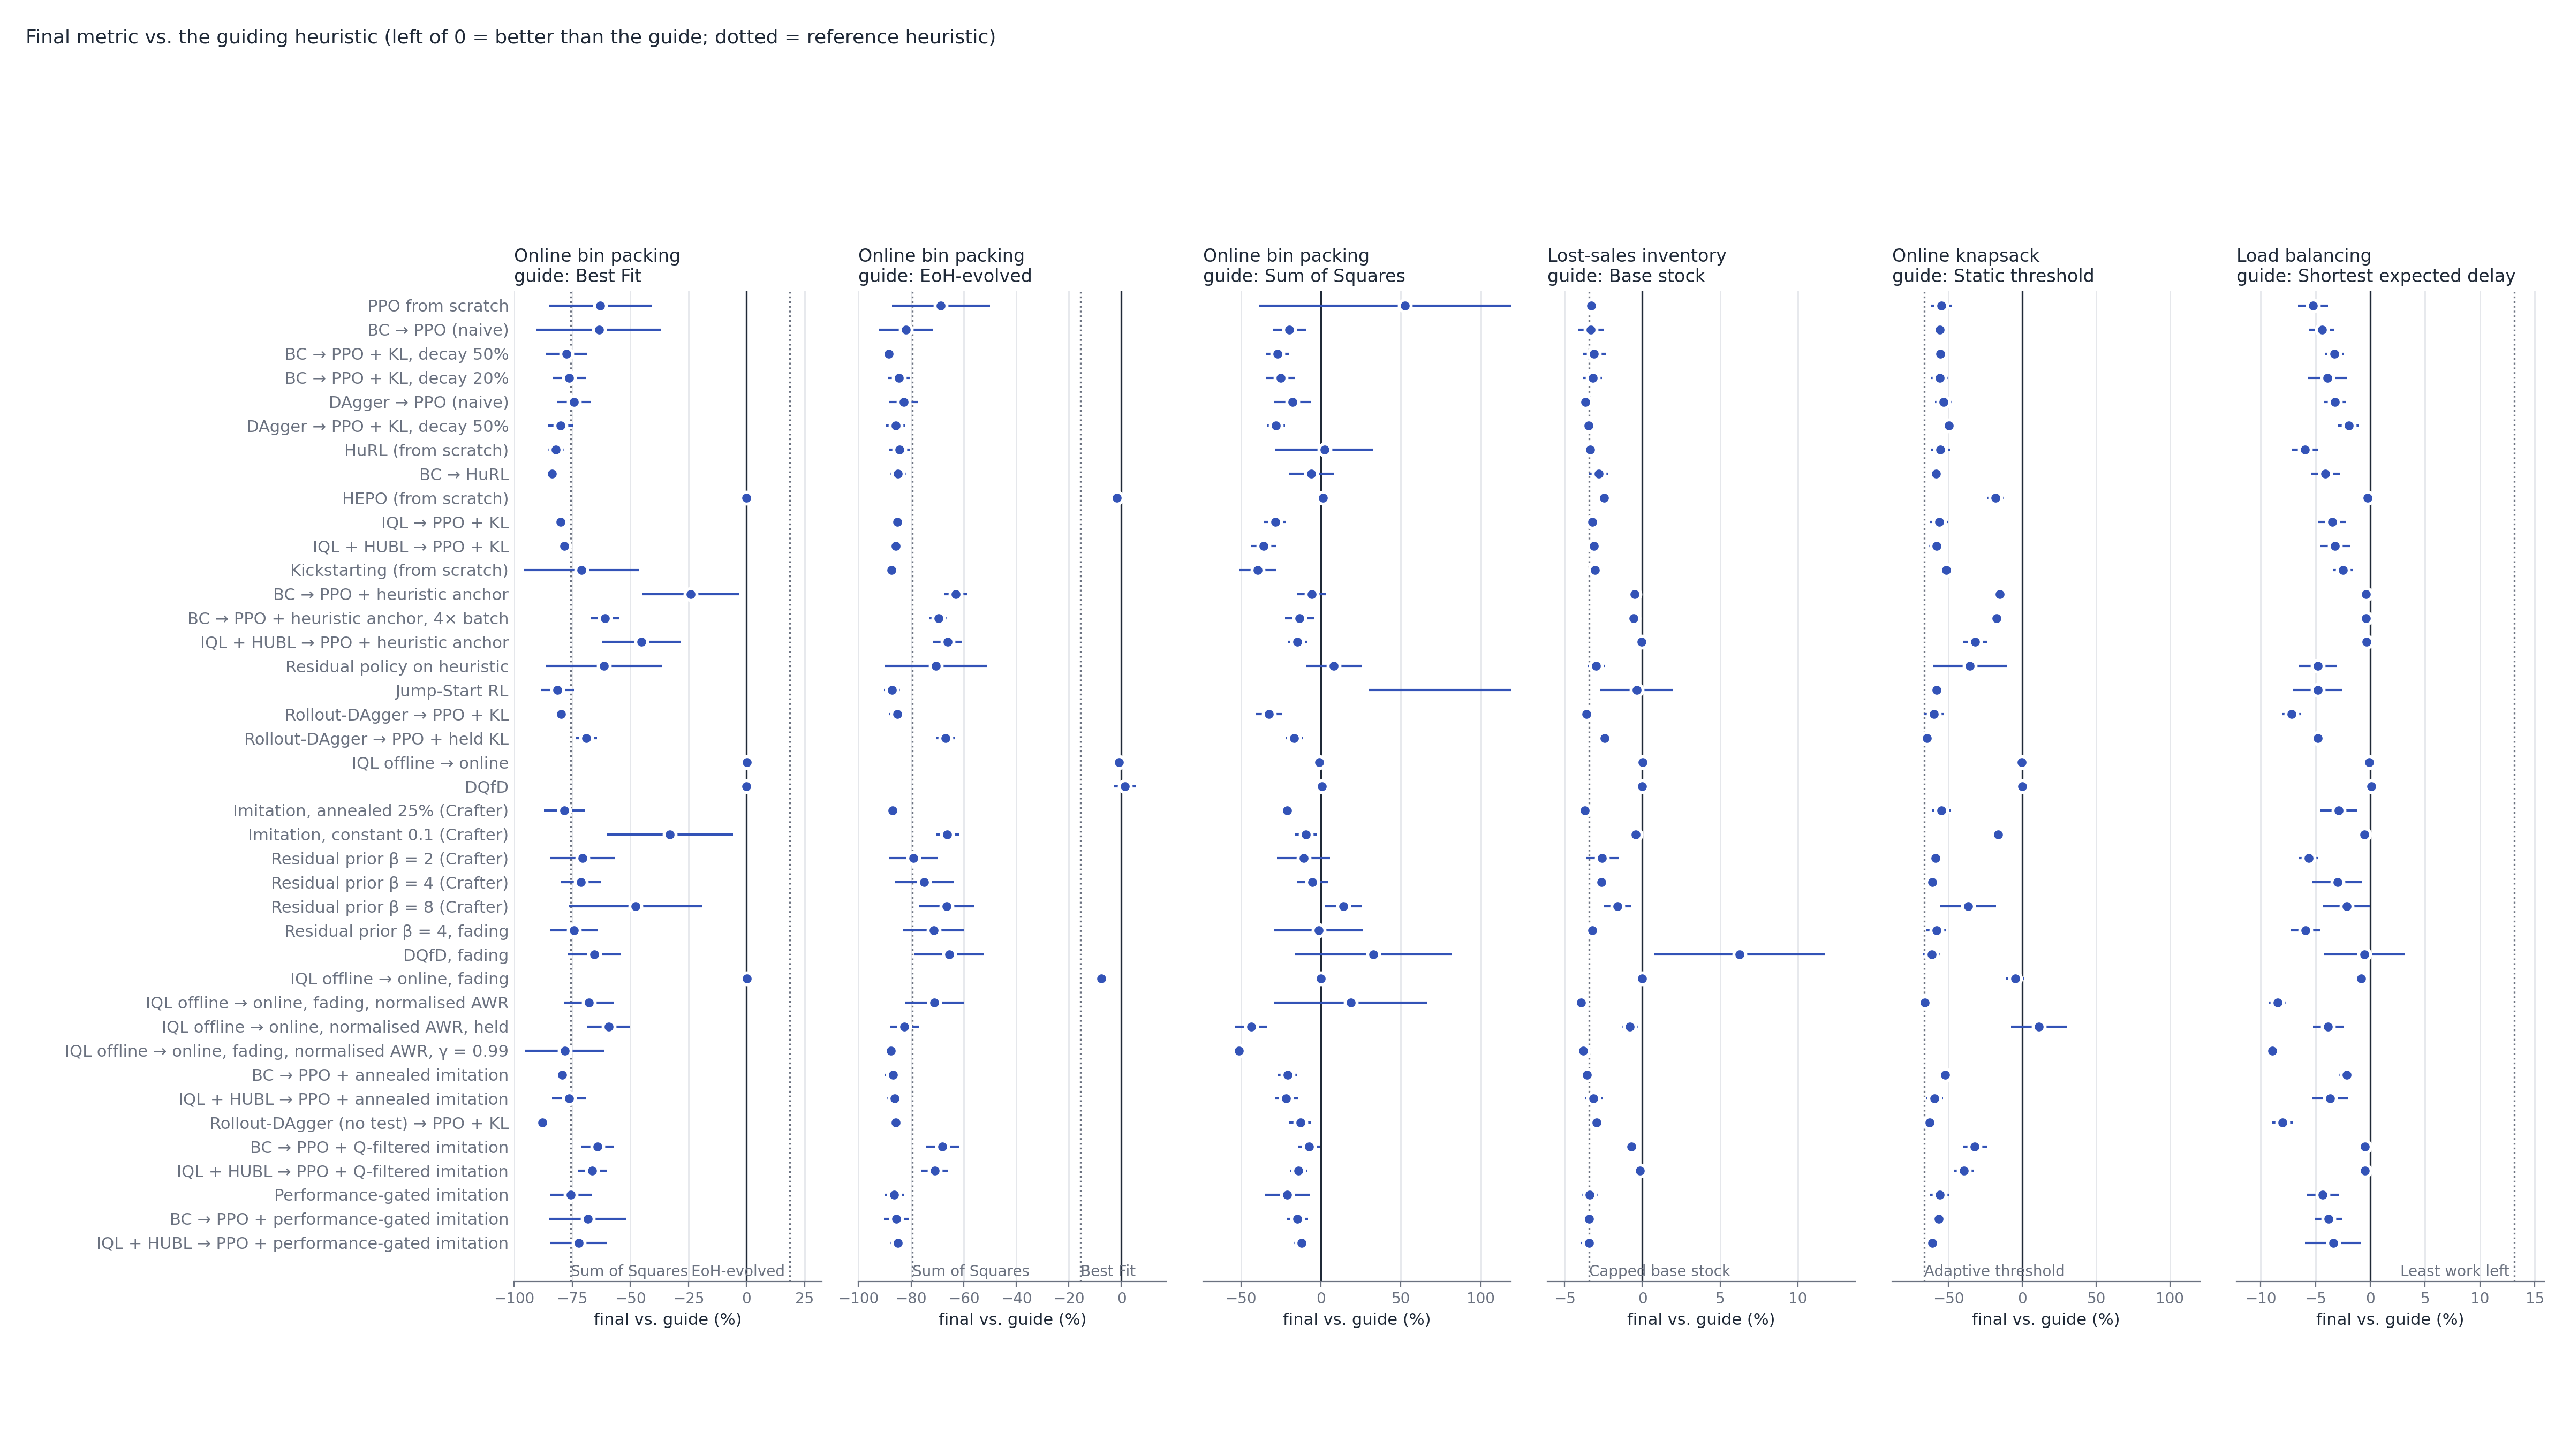
\includegraphics[width=\linewidth]{overview.png}
\caption{Final metric relative to the guide heuristic (mean $\pm$ std over 10 seeds; left of 0 is better than the
guide; the axis is cut at $+100\%$). Dotted: reference heuristics within the plotted range.}
\label{fig:overview}
\end{sidewaysfigure}

\begin{figure}[p]
\centering
\begin{subfigure}{0.49\linewidth}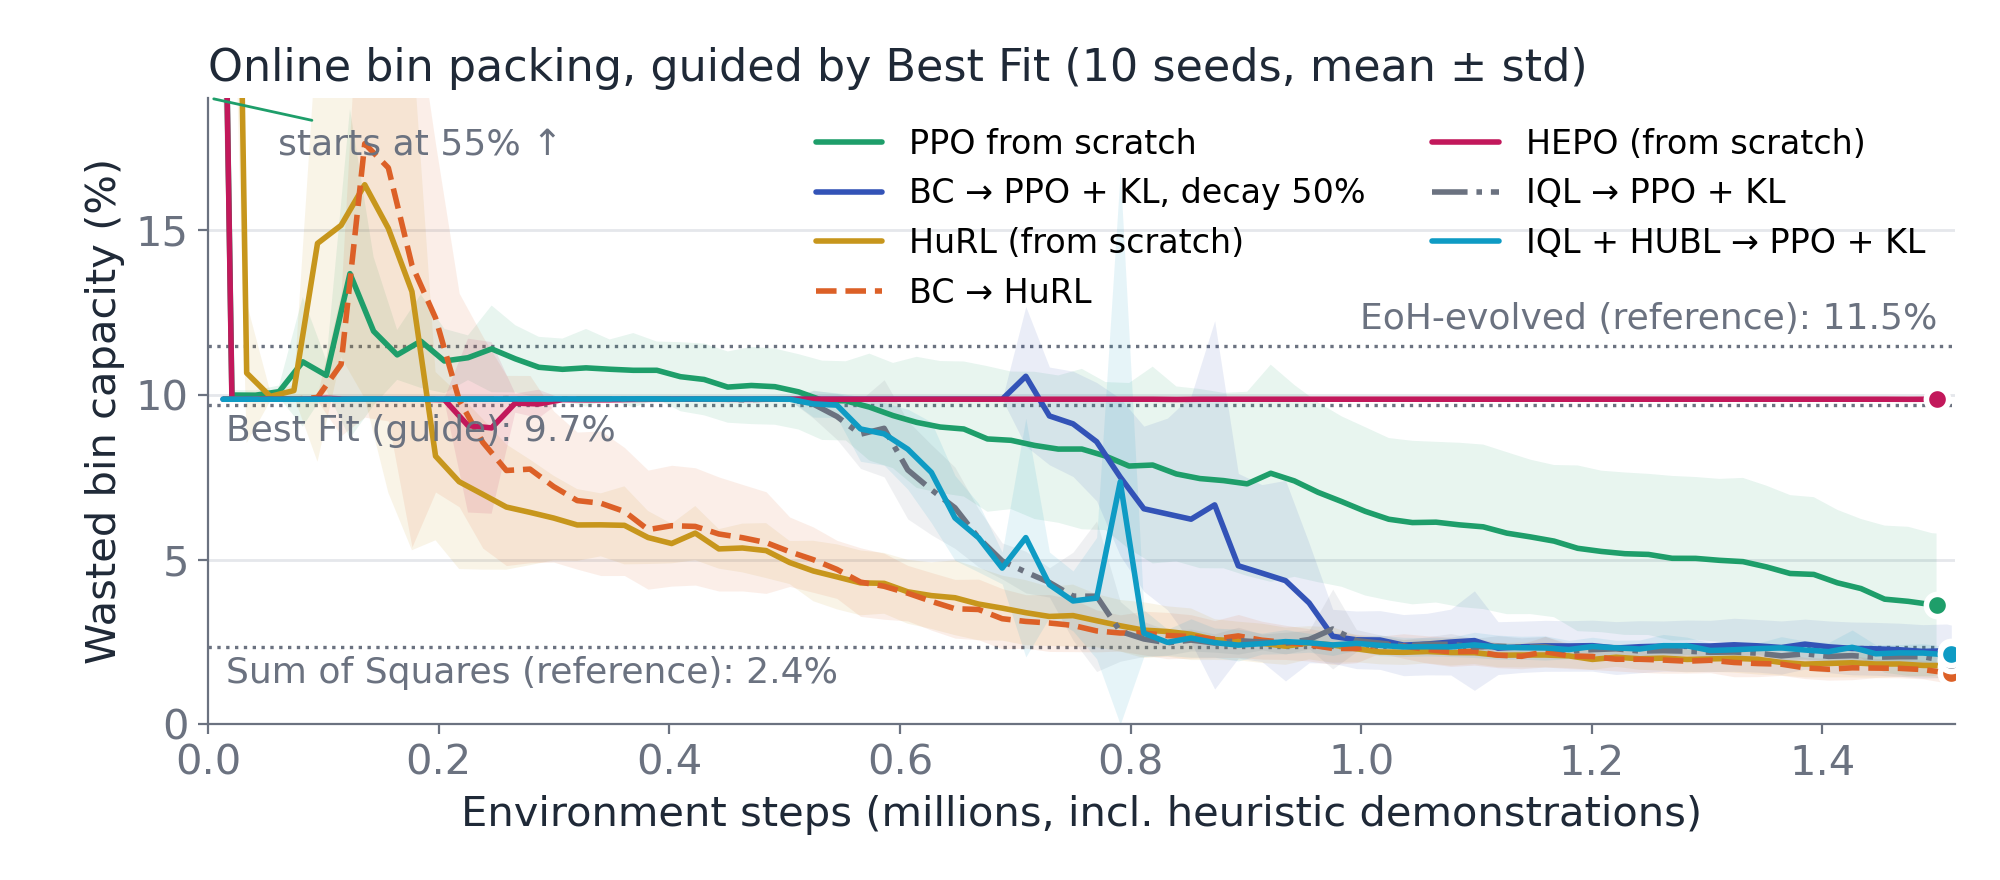
\includegraphics[width=\linewidth]{binpack_toy/best_fit/learning_curves_guided.png}\end{subfigure}
\begin{subfigure}{0.49\linewidth}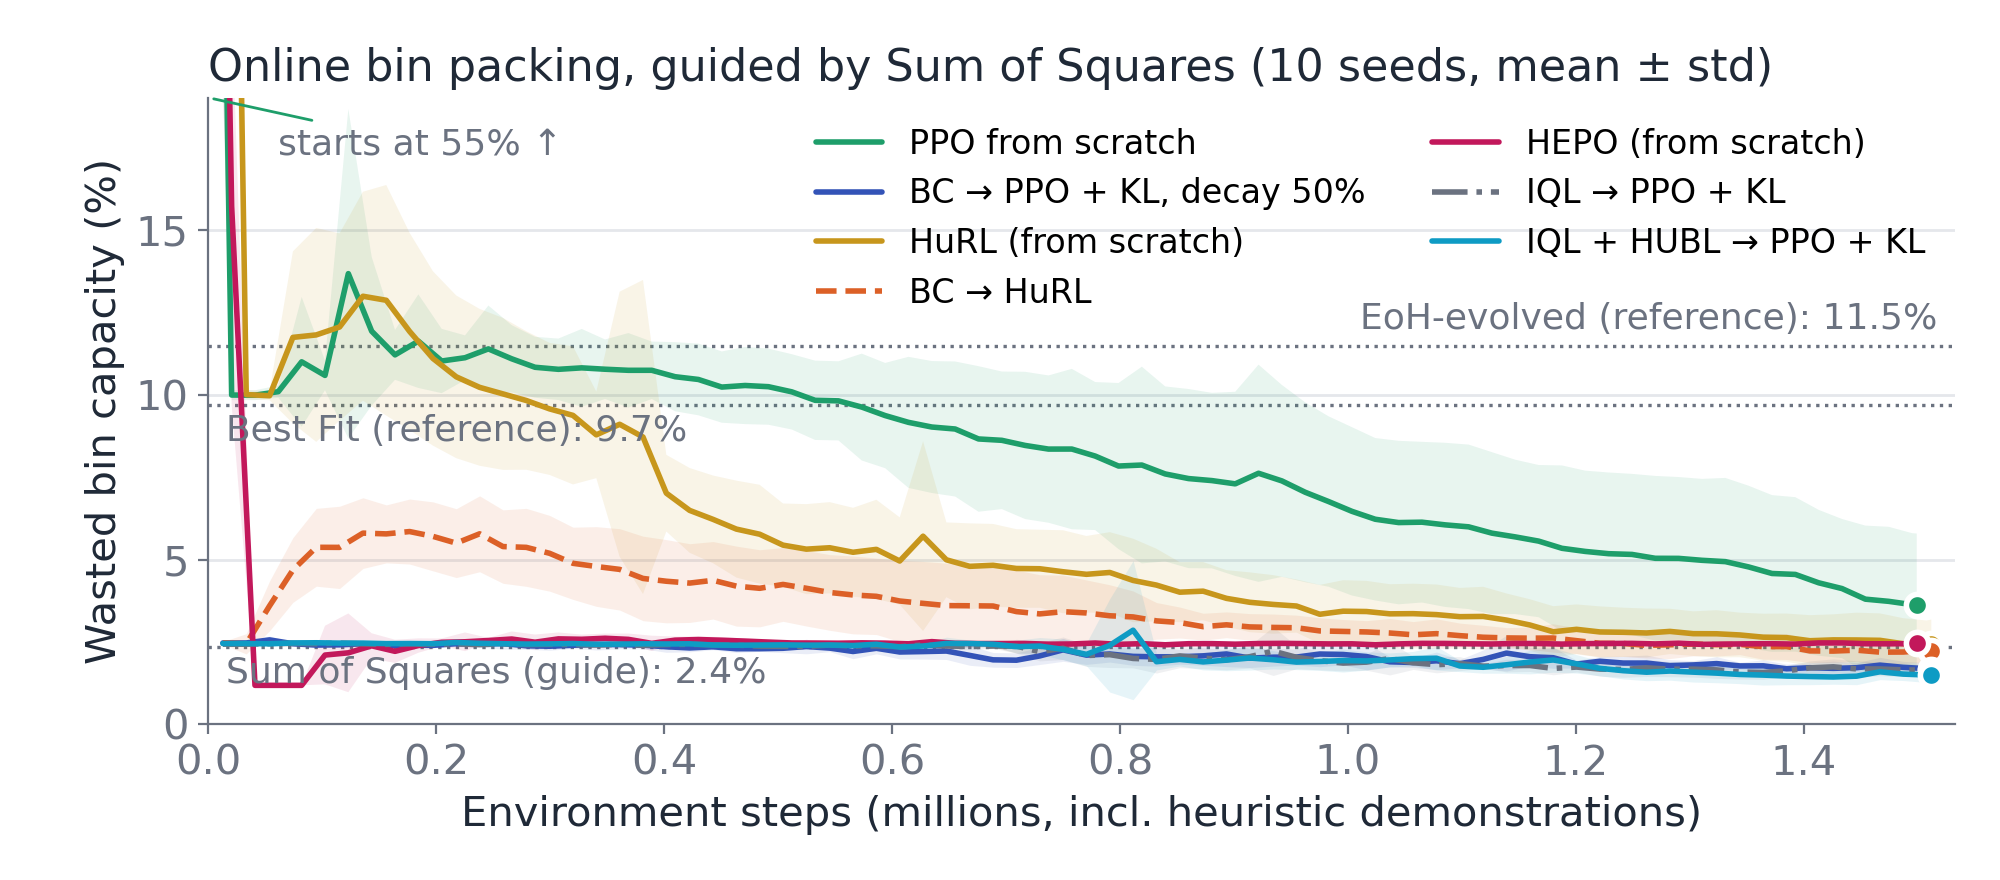
\includegraphics[width=\linewidth]{binpack_toy/sum_of_squares/learning_curves_guided.png}\end{subfigure}
\begin{subfigure}{0.49\linewidth}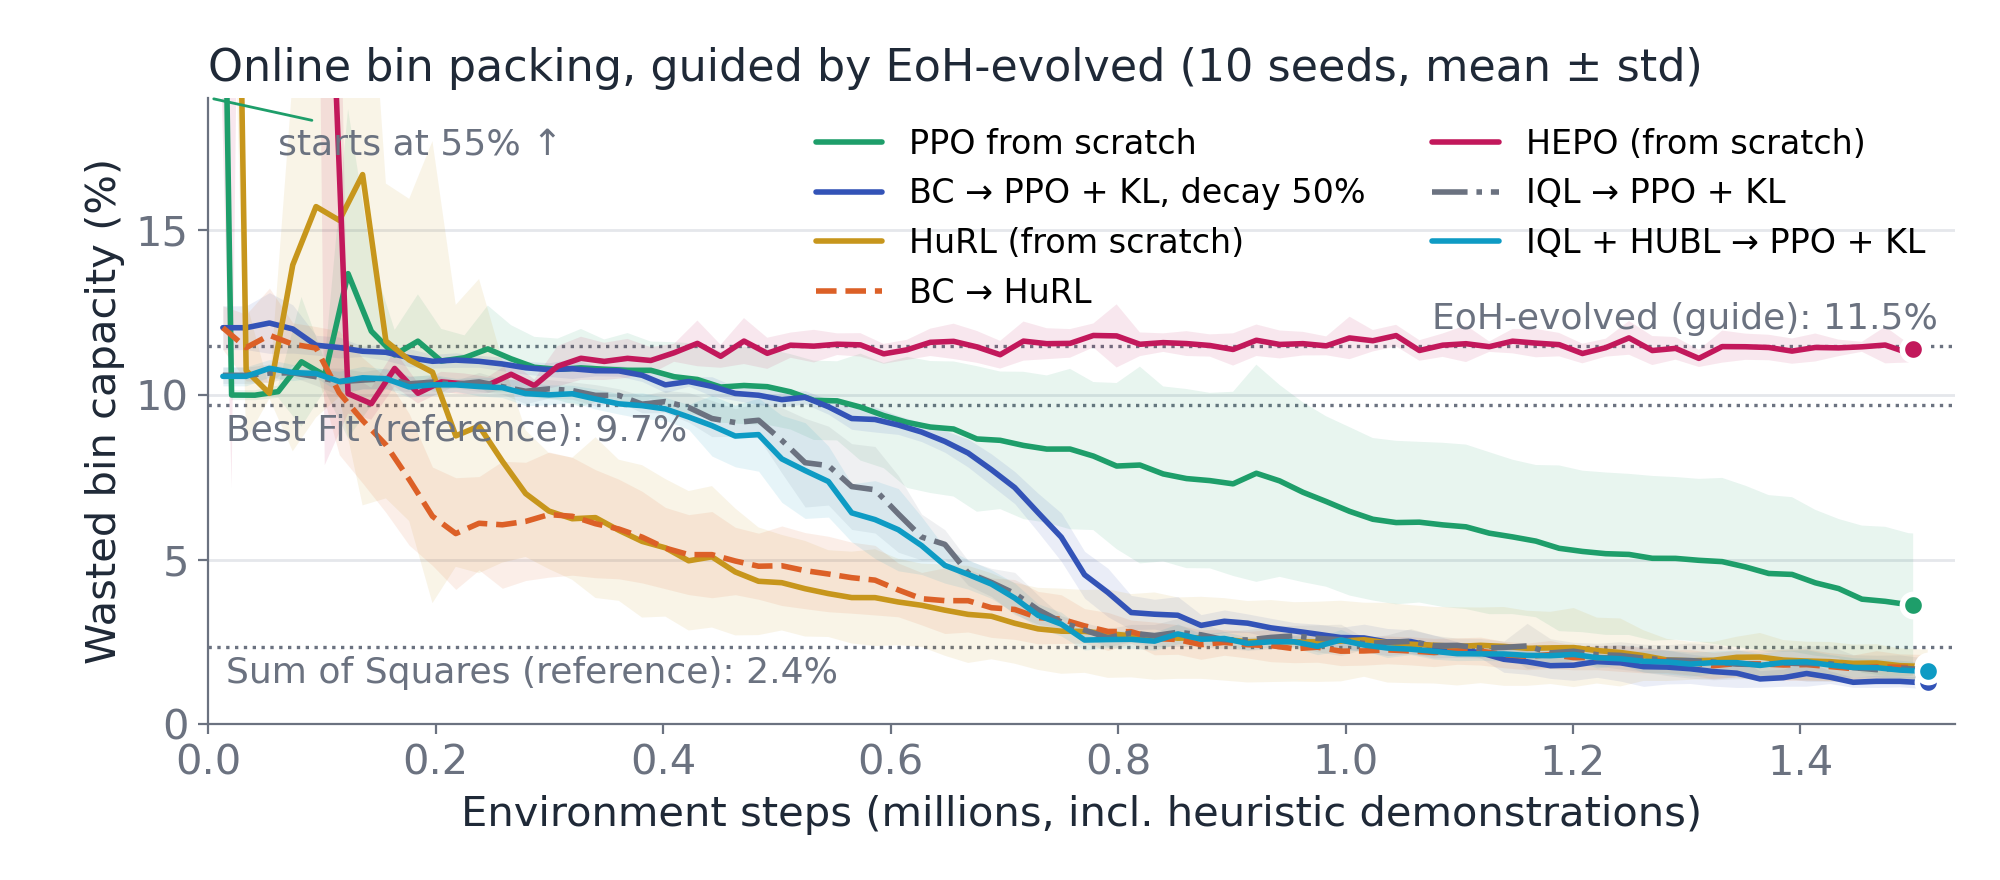
\includegraphics[width=\linewidth]{binpack_toy/eoh_evolved/learning_curves_guided.png}\end{subfigure}
\begin{subfigure}{0.49\linewidth}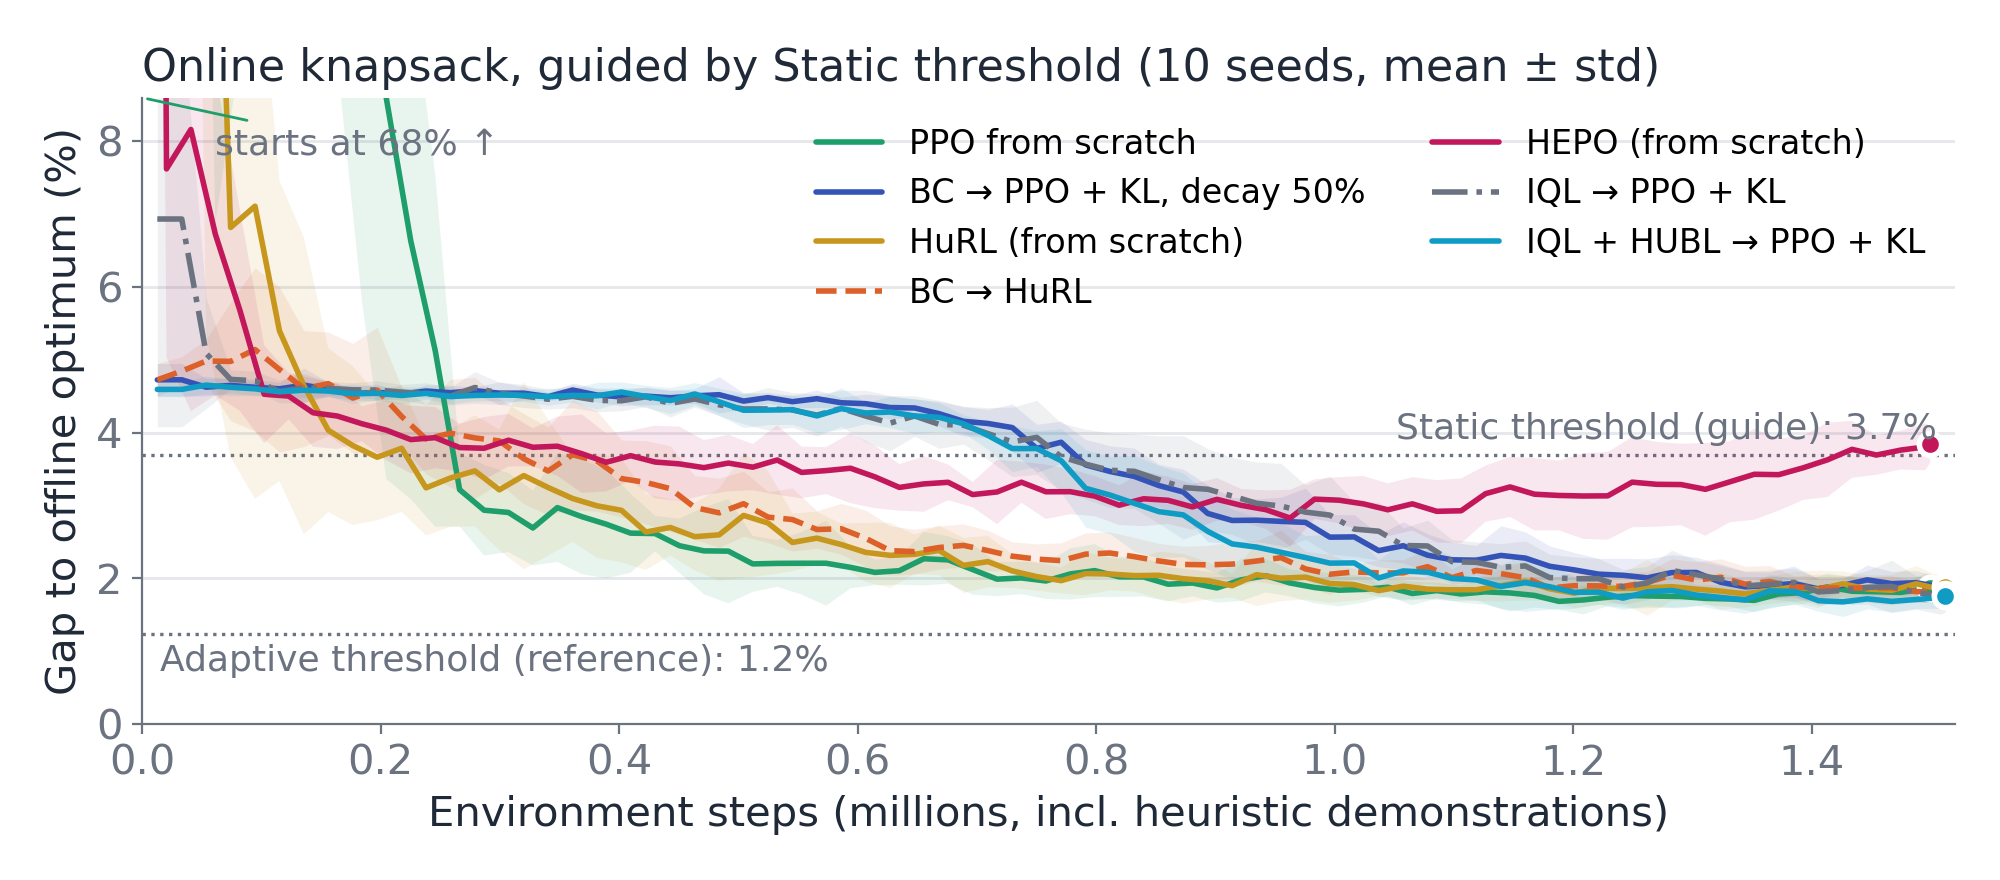
\includegraphics[width=\linewidth]{knapsack/static_threshold/learning_curves_guided.png}\end{subfigure}
\begin{subfigure}{0.49\linewidth}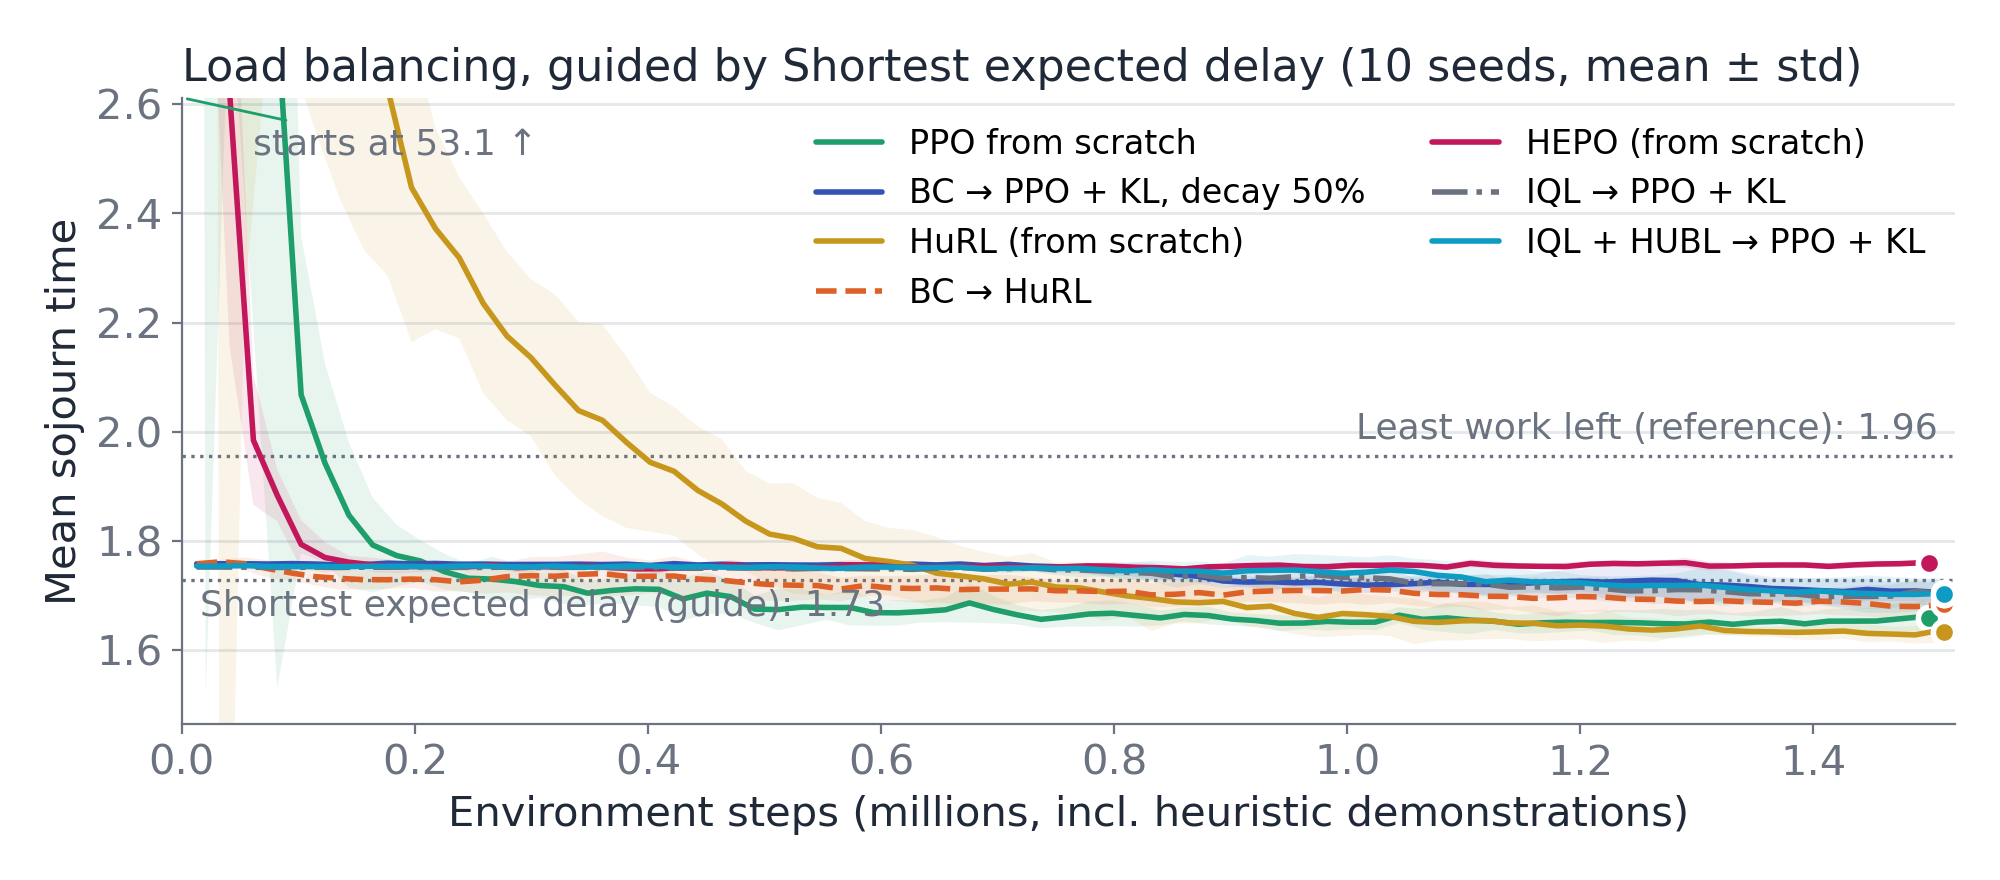
\includegraphics[width=\linewidth]{load_balancing/shortest_expected_delay/learning_curves_guided.png}\end{subfigure}
\begin{subfigure}{0.49\linewidth}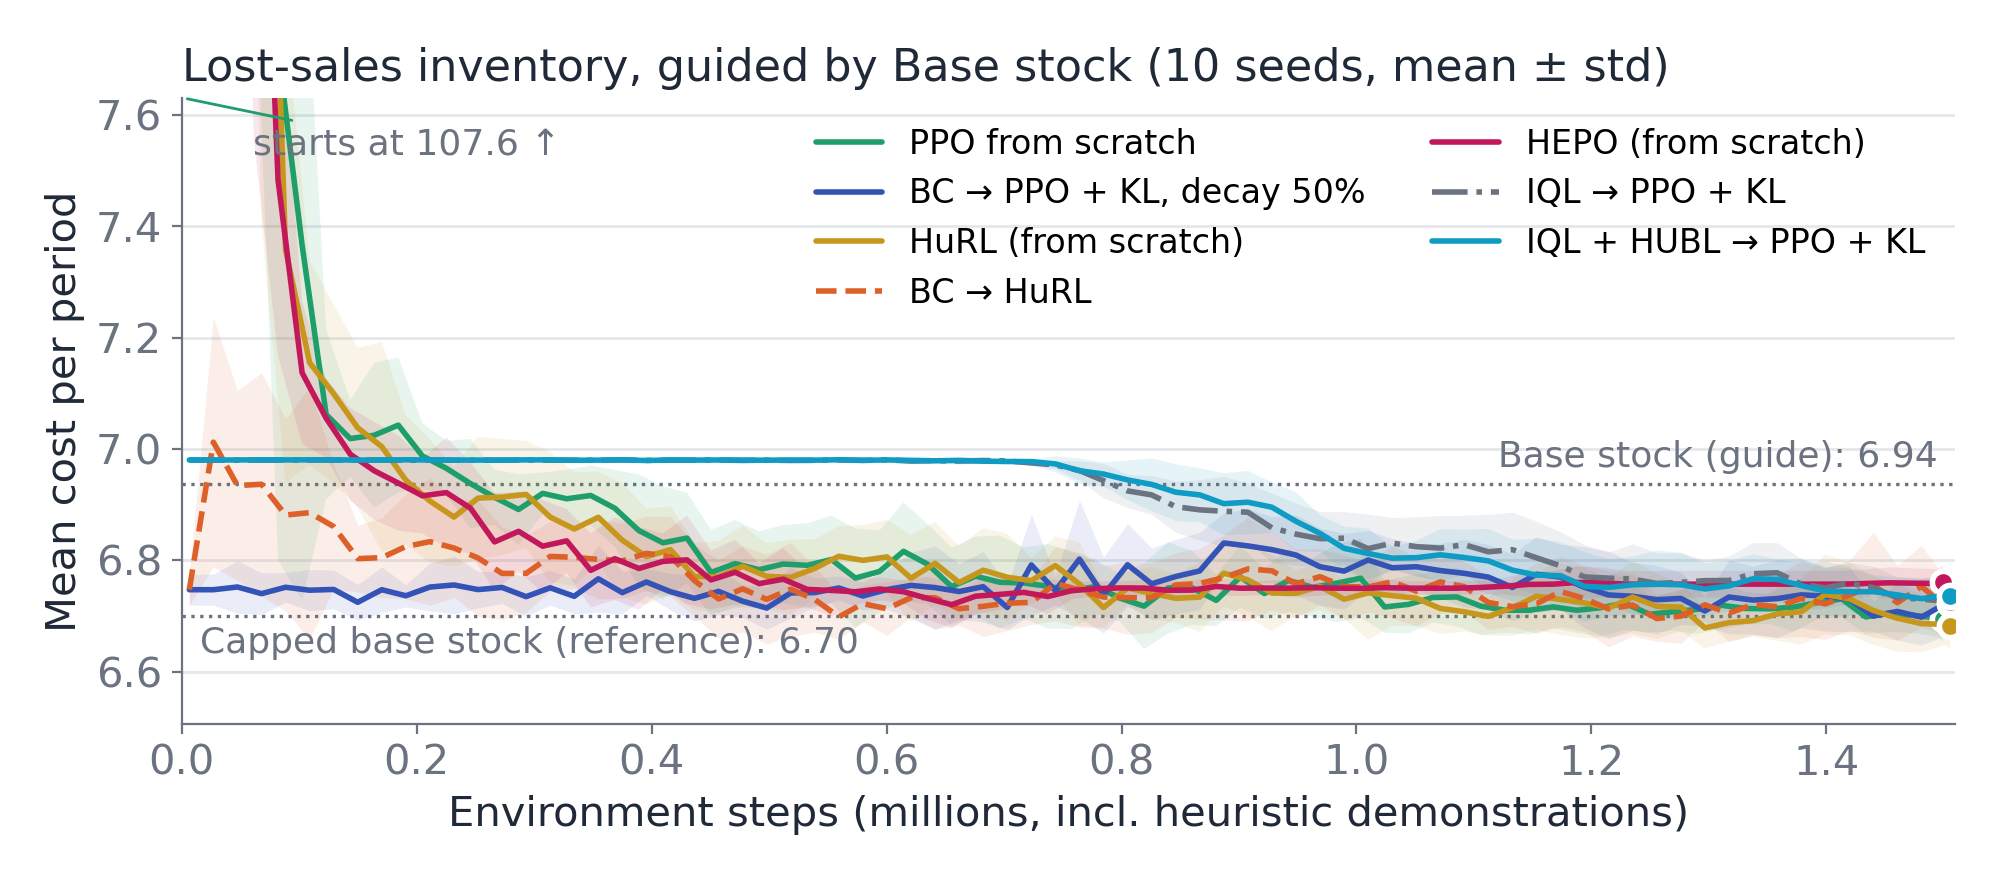
\includegraphics[width=\linewidth]{inventory/base_stock/learning_curves_guided.png}\end{subfigure}
\caption{Learning curves of the offline warm starts and HuRL/HEPO against PPO from scratch (mean $\pm$ std over
10 seeds; the x-axis includes the heuristic's demonstration steps).}
\label{fig:curves}
\end{figure}

\begin{figure}[p]
\centering
\begin{subfigure}{0.49\linewidth}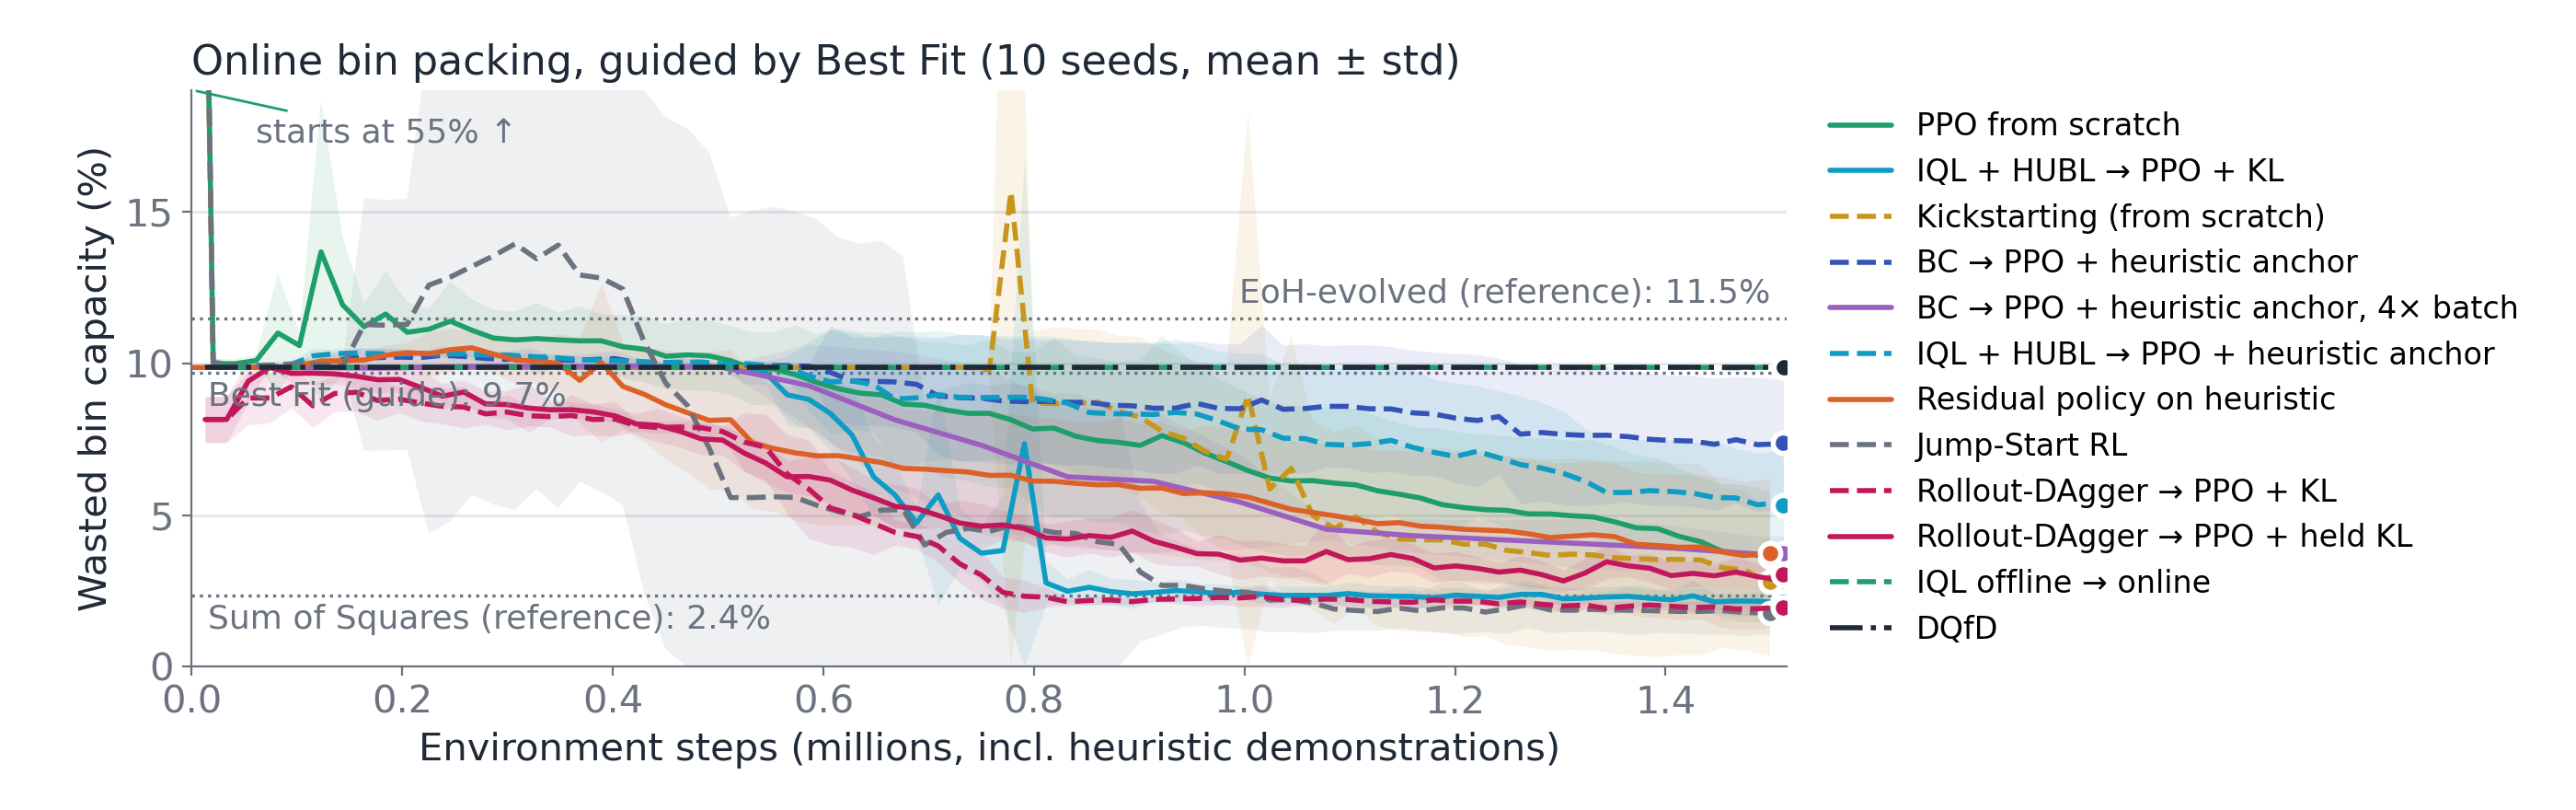
\includegraphics[width=\linewidth]{binpack_toy/best_fit/learning_curves_online.png}\end{subfigure}
\begin{subfigure}{0.49\linewidth}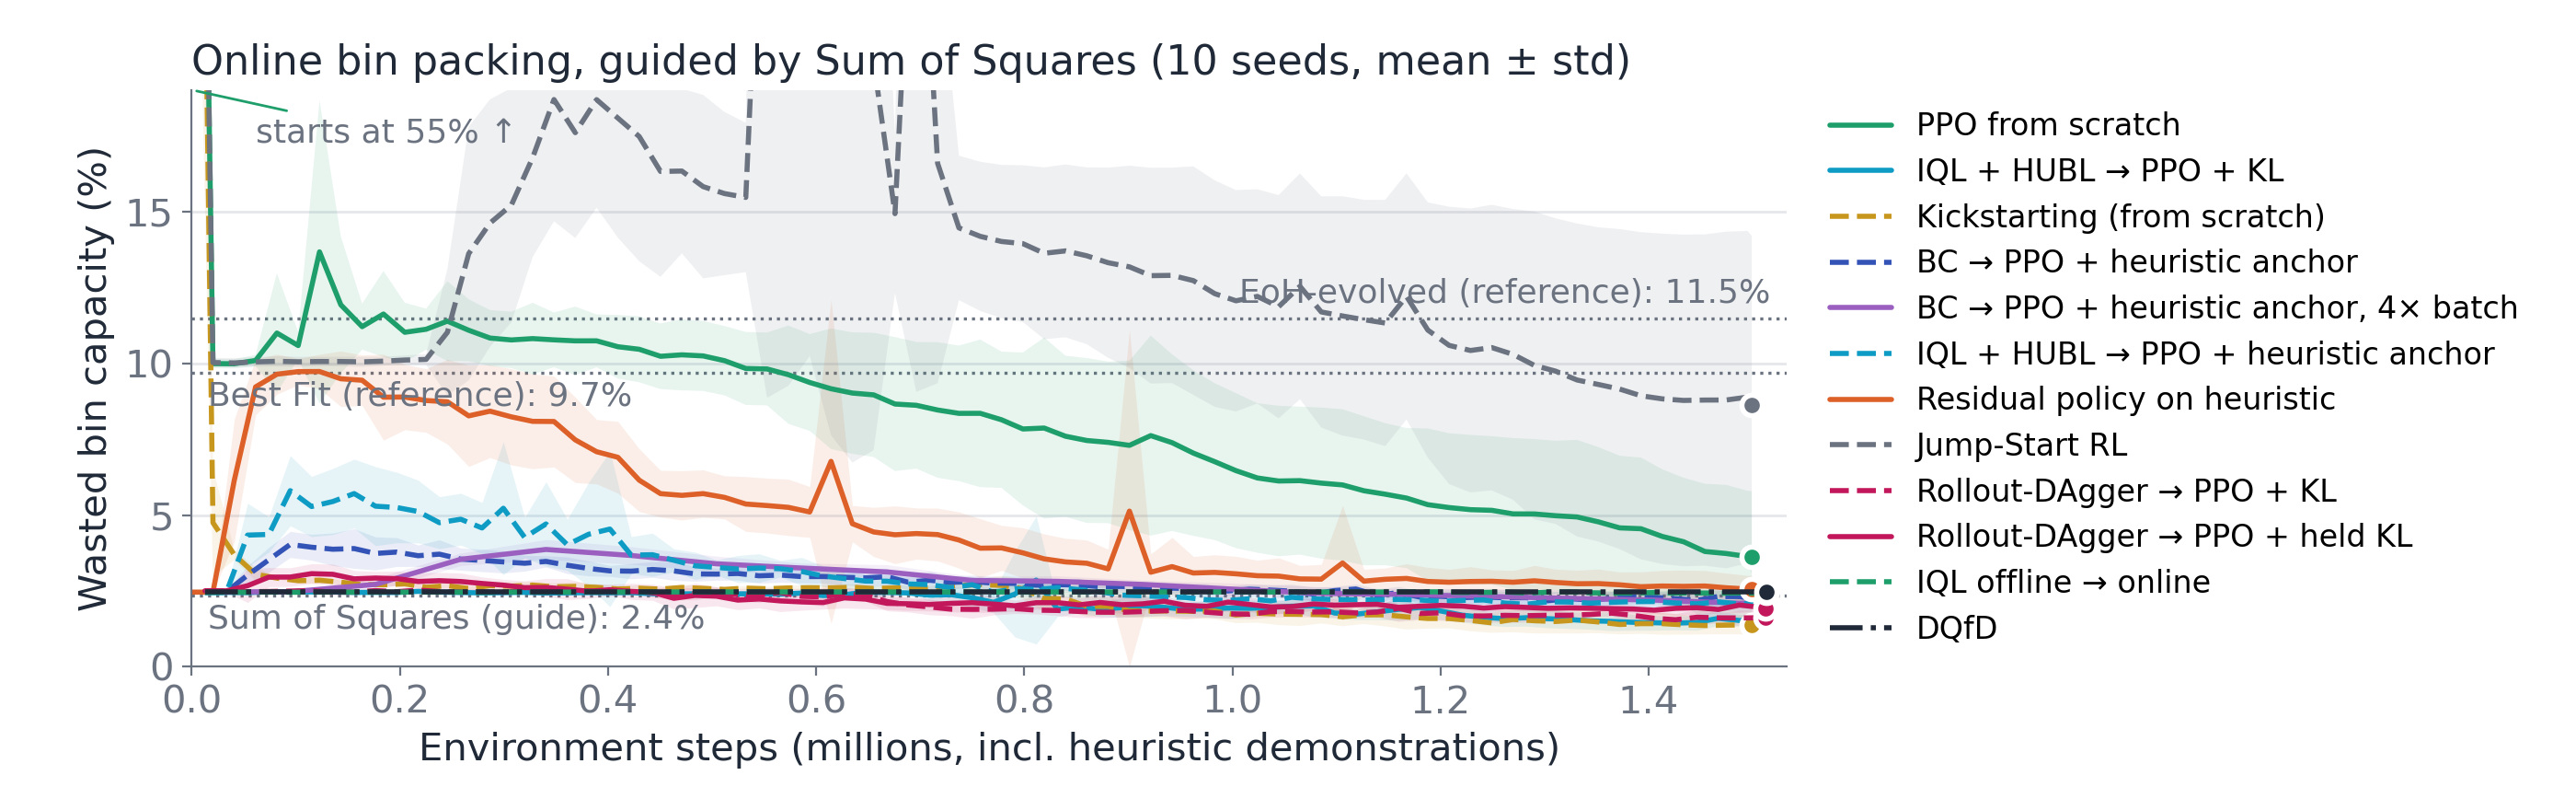
\includegraphics[width=\linewidth]{binpack_toy/sum_of_squares/learning_curves_online.png}\end{subfigure}
\begin{subfigure}{0.49\linewidth}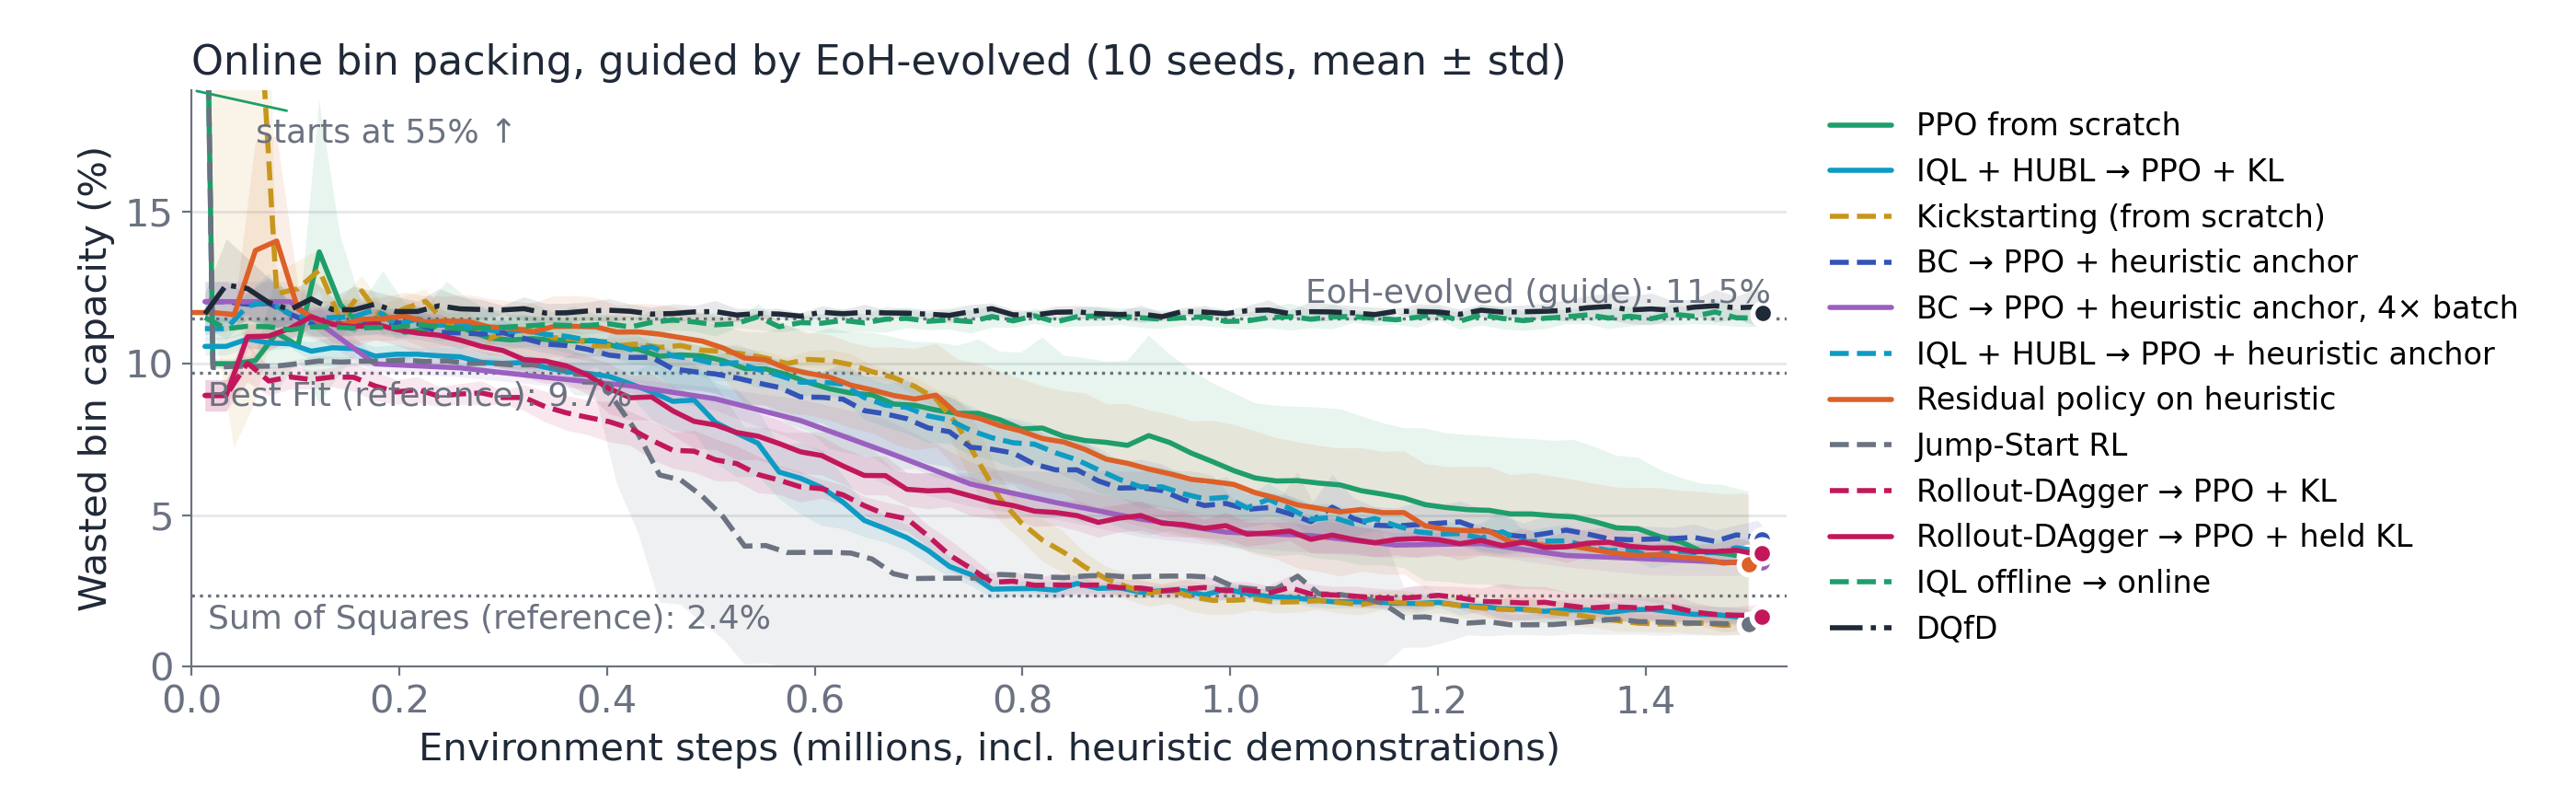
\includegraphics[width=\linewidth]{binpack_toy/eoh_evolved/learning_curves_online.png}\end{subfigure}
\begin{subfigure}{0.49\linewidth}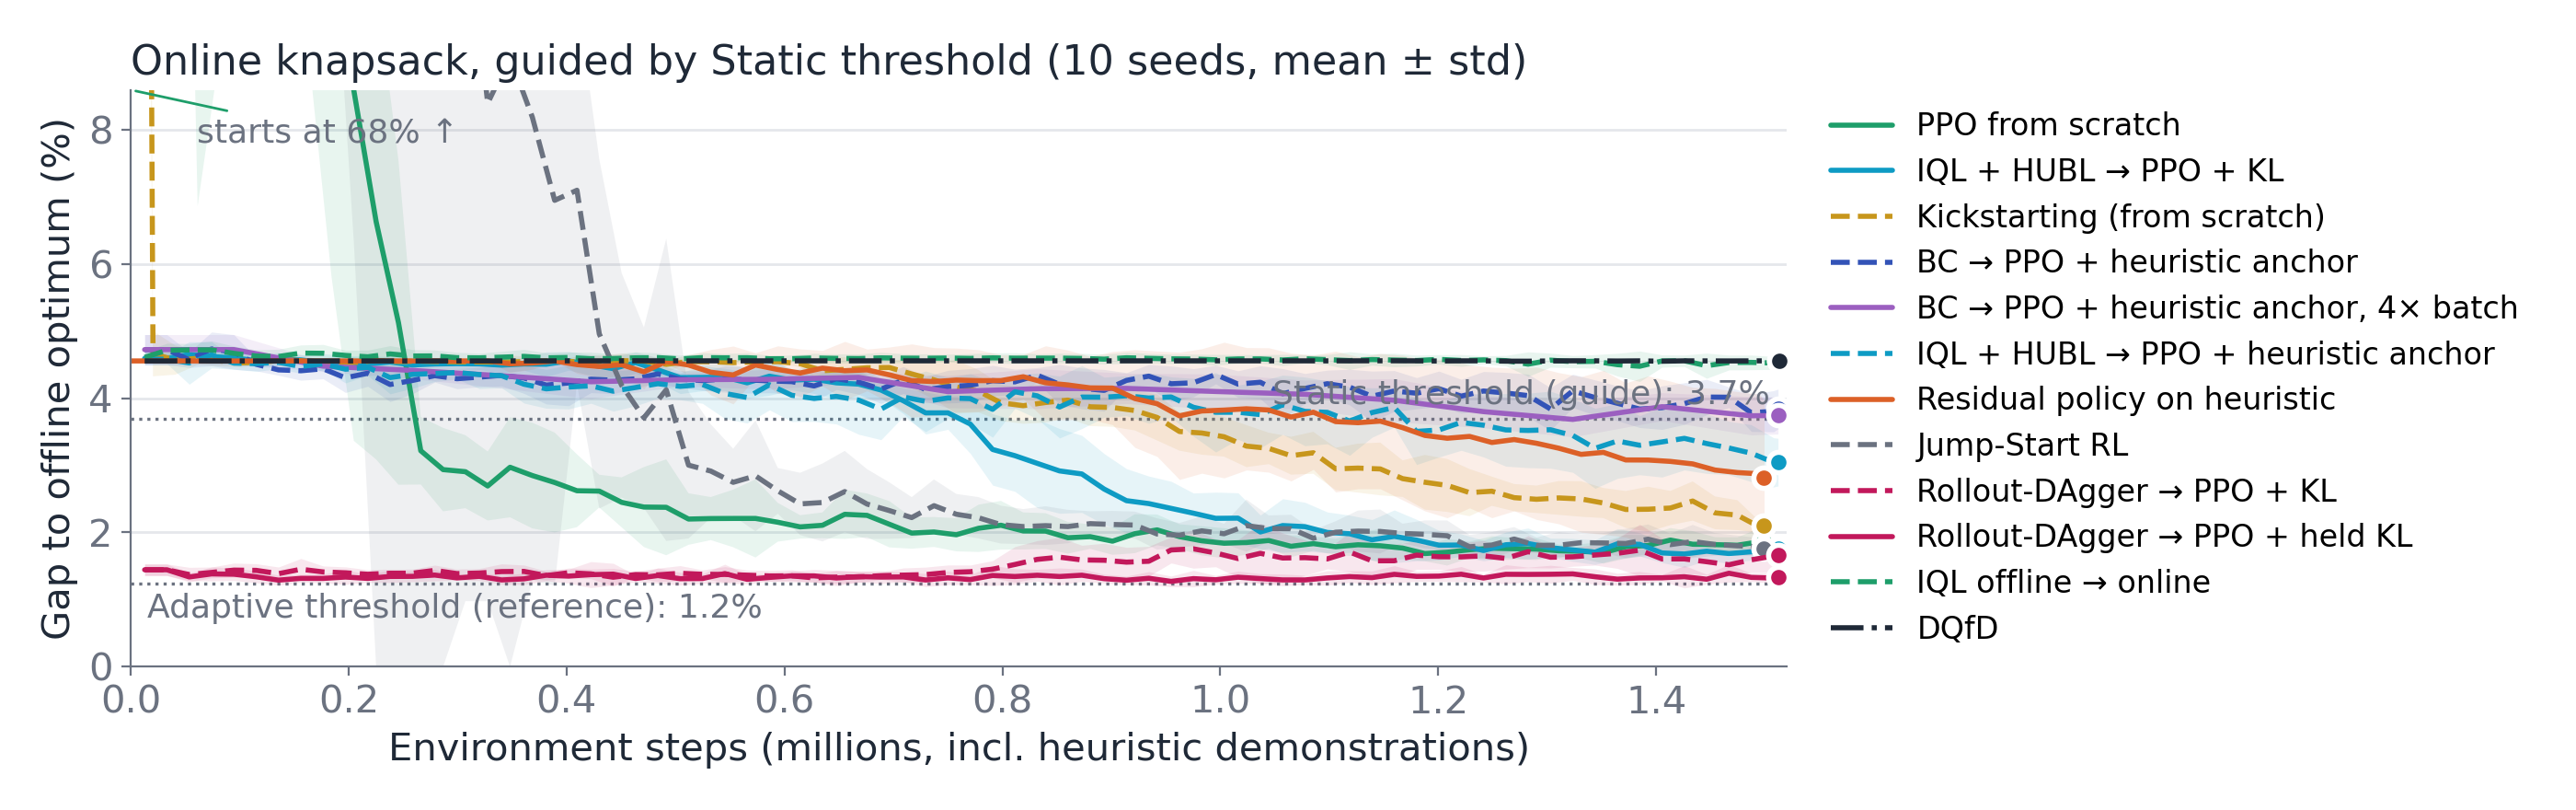
\includegraphics[width=\linewidth]{knapsack/static_threshold/learning_curves_online.png}\end{subfigure}
\begin{subfigure}{0.49\linewidth}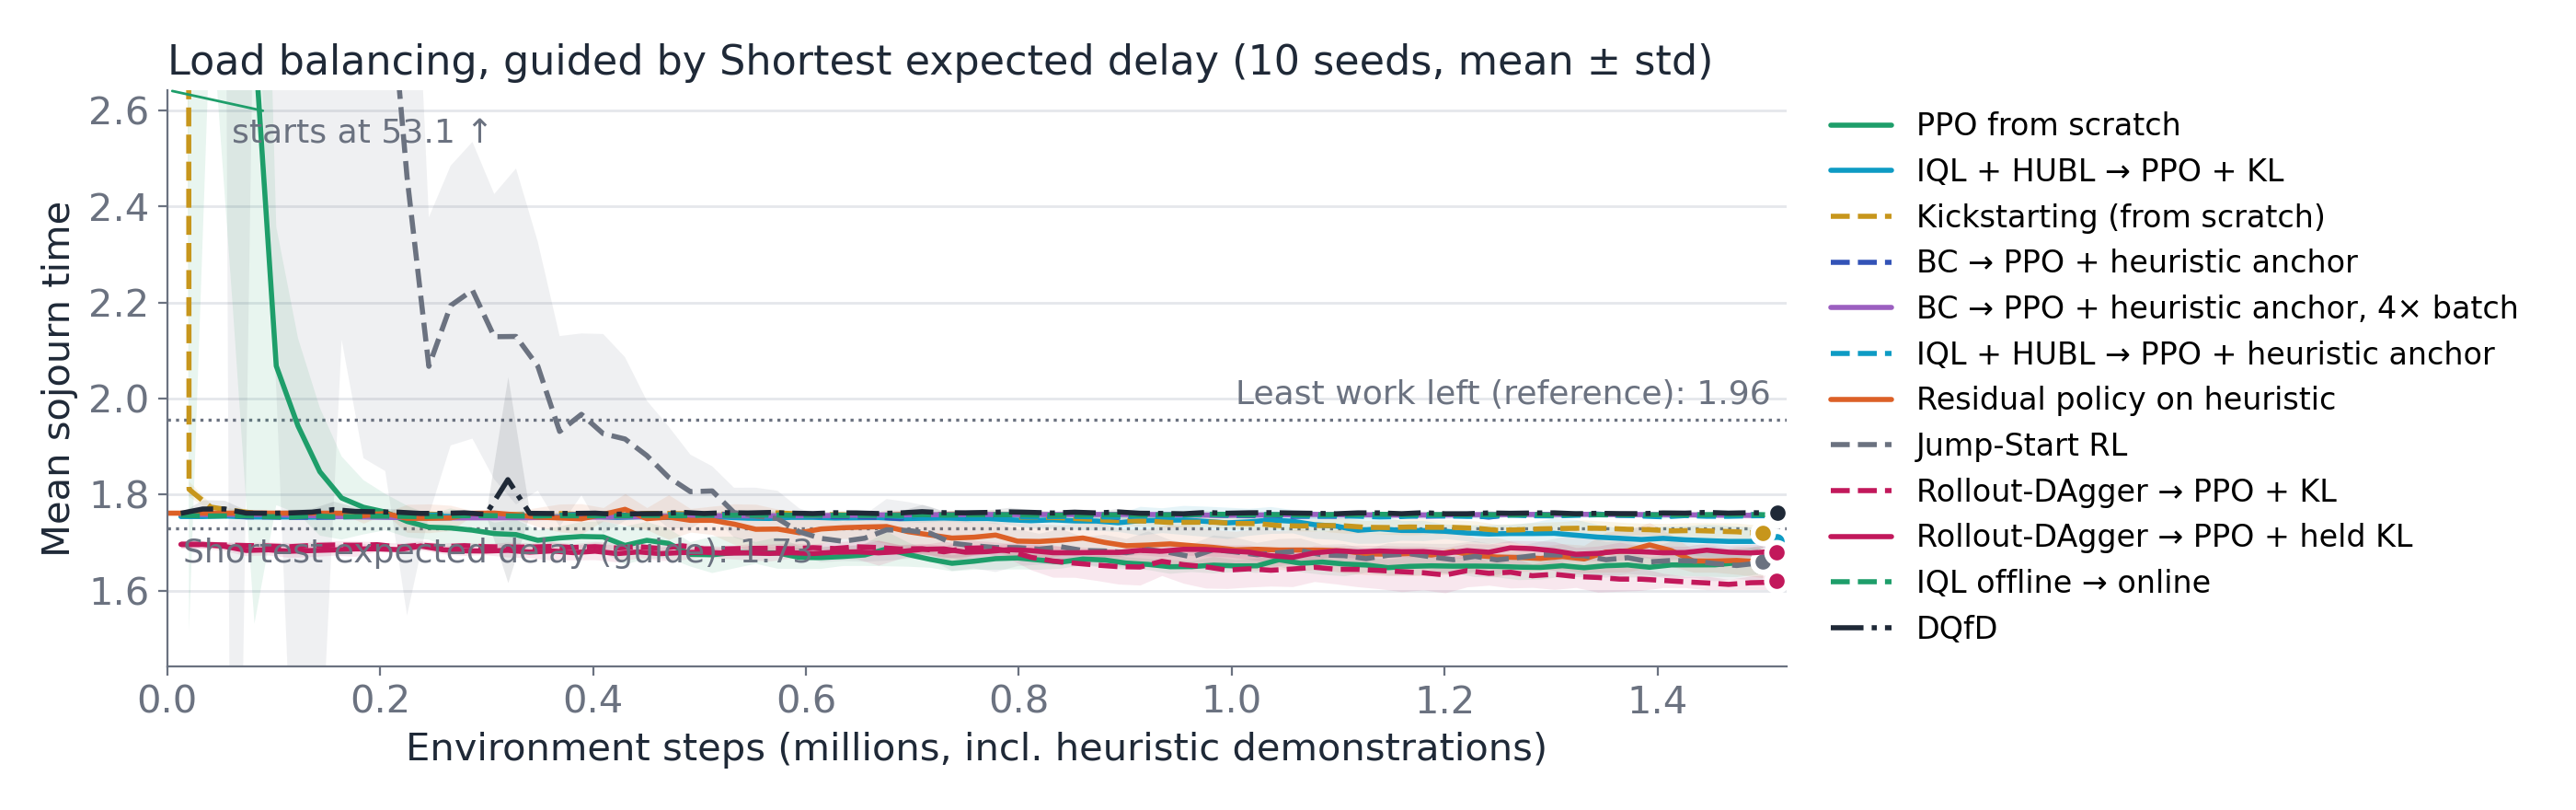
\includegraphics[width=\linewidth]{load_balancing/shortest_expected_delay/learning_curves_online.png}\end{subfigure}
\begin{subfigure}{0.49\linewidth}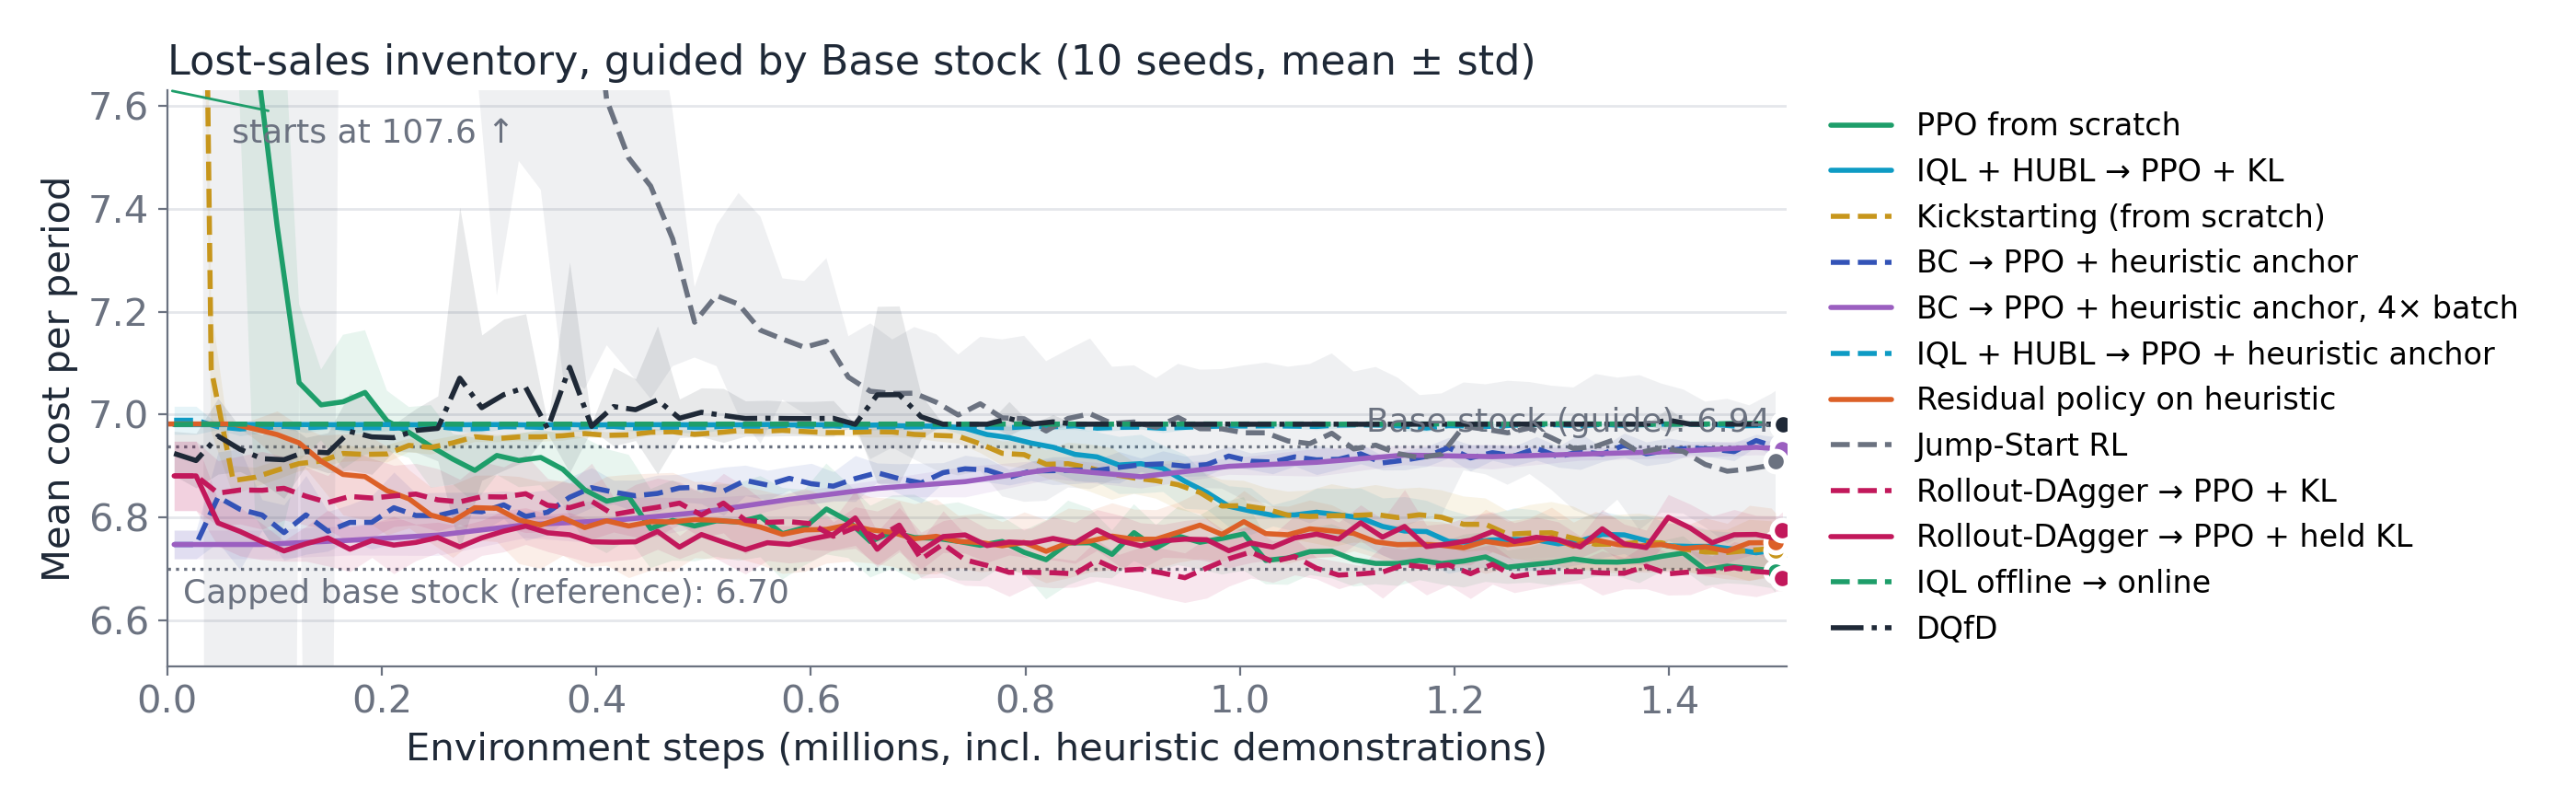
\includegraphics[width=\linewidth]{inventory/base_stock/learning_curves_online.png}\end{subfigure}
\caption{Learning curves of the methods that use the heuristic during RL, Rollout-DAgger and the off-policy methods,
against PPO from scratch and IQL + HUBL $\to$ PPO + KL.}
\label{fig:curves-online}
\end{figure}

Table~\ref{tab:scorecard} answers the three questions per method and experiment; Table~\ref{tab:final} gives the
final metric (Q1, Q3), Table~\ref{tab:beat} the steps to beat the guide (Q2), and Table~\ref{tab:rollout} the
rollout-improved heuristics. Figure~\ref{fig:overview} shows every final result relative to its guide, and
Figures~\ref{fig:curves} and~\ref{fig:curves-online} the learning curves.

\paragraph{Overall ranking.} Ranking the 21 methods by final metric in each experiment and averaging over the six:
Rollout-DAgger $\to$ PPO + KL 3.3; IQL + HUBL $\to$ PPO + KL and IQL $\to$ PPO + KL 6.5; HuRL 7.5; BC $\to$ HuRL,
BC $\to$ PPO + KL and DAgger $\to$ PPO + KL 7.7; \dots; PPO from scratch 11.5; residual policy 13.2; the three
constant-anchor variants 15.3--17.2; HEPO 17.5; IQL offline $\to$ online 19.5; DQfD 19.8.
Among all 40 methods, including those of Section~\ref{sec:followup}: Rollout-DAgger $\to$ PPO + KL 6.8; online IQL
with normalised advantage weights and $\gamma = 0.99$ 9.5; Rollout-DAgger without the significance test 10.2;
performance-gated imitation 12.2; IQL + HUBL $\to$ PPO + annealed imitation 12.3; IQL and IQL + HUBL $\to$ PPO + KL
12.5; annealed imitation (Crafter) 12.7; \dots; PPO from scratch 23.3.

\paragraph{Q1: better than PPO from scratch?} Often on bin packing, rarely elsewhere.
\begin{itemize}[leftmargin=*]
\item PPO from scratch is unreliable on bin packing: 3.59 $\pm$ 2.14\% over 10 seeds, with single seeds between
  about 1.8\% and 6\%. Most warm starts are significantly better there with Sum of Squares and EoH as guide, and
  about half of them with Best Fit, mainly by being consistent (e.g.\ IQL + HUBL $\to$ PPO + KL 1.51 $\pm$ 0.18\%
  with Sum of Squares).
\item Rollout-DAgger $\to$ PPO + KL is significantly better in four experiments (the three bin-packing guides and load
  balancing, 1.60 vs 1.64) and never worse. IQL and IQL + HUBL $\to$ PPO + KL are better in three and worse in one
  (load balancing, 1.67 vs 1.64).
\item On knapsack, load balancing and inventory PPO from scratch is already good, and most methods are within noise
  of it or worse. Exceptions: Rollout-DAgger $\to$ PPO + held KL on knapsack (1.30 vs 1.67\%, the best knapsack
  result, close to the adaptive-threshold reference 1.24\%) and DAgger $\to$ PPO on inventory (6.68 vs 6.71).
\item Methods that hold the policy at the heuristic for the whole run are significantly \emph{worse} than PPO from
  scratch in three to five experiments: the three constant-anchor variants (3--4), HEPO, DQfD and IQL offline $\to$
  online (5 each).
\item Most offline warm starts are slightly but significantly worse on load balancing (1.66--1.69 vs 1.64), where PPO
  from scratch is already better than the guide after 174k steps.
\end{itemize}

\paragraph{Q2: reaches the heuristic's level faster?} Yes, for nearly every method that starts from the heuristic.
\begin{itemize}[leftmargin=*]
\item Rollout-DAgger, IQL and IQL + HUBL $\to$ PPO + KL beat the guide sooner than PPO from scratch in all six
  experiments. Rollout-DAgger starts below the guide in five of six (its clone already improves on it: knapsack
  1.44\% before any RL) and beats Best Fit after 13k steps instead of 635k.
\item With a strong guide the gain is large (load balancing 13k vs 174k steps, inventory 6k vs 133k, Sum of Squares
  23--136k vs 1372k for most warm starts).
\item With a weak guide, cloning is not faster: with Best Fit, BC $\to$ PPO and BC $\to$ PPO + KL need 730--740k
  steps against 635k, because the clone starts at Best Fit and has to unlearn it. With the even weaker EoH guide Q2 is
  trivial: PPO from scratch passes it after 20k steps.
\item Methods without a warm start (HuRL, kickstarting, HEPO, Jump-Start RL) are faster in some experiments only.
  Jump-Start RL never passes Sum of Squares.
\item Methods that start at the guide get Q2 credit from the first evaluation below it on 64 episodes, which can be
  noise: DQfD and IQL offline $\to$ online are marked faster in several experiments although they end at the guide.
\end{itemize}

\paragraph{Q3: better than the heuristic?} Yes for nearly every method that lets the heuristic go.
\begin{itemize}[leftmargin=*]
\item The BC, DAgger and IQL warm starts, kickstarting and Rollout-DAgger end significantly better than the guide in
  all six experiments; HuRL, BC $\to$ HuRL and PPO from scratch in five (not with Sum of Squares); the residual
  policy in five, Jump-Start RL and HEPO in four.
\item How far beyond: on bin packing the best methods end at 1.3--1.6\% waste whatever the guide, 30--45\% below Sum
  of Squares and far below Best Fit and EoH. The guide's quality hardly changes the final level here; the weak EoH
  guide gave the best bin-packing result of the 21 main methods (BC $\to$ PPO + KL 1.32 $\pm$ 0.14\%;
  Section~\ref{sec:followup} has better ones: 1.18\% with Best Fit, 1.15\% with Sum of Squares). On inventory all good methods
  reach capped base stock (6.68--6.72 vs 6.70); on knapsack only Rollout-DAgger $\to$ PPO + held KL approaches the
  adaptive threshold.
\item The methods that hold the heuristic end at it or barely below it: DQfD and IQL offline $\to$ online are
  never significantly better than the guide (DQfD ends exactly at Best Fit, 9.68 $\pm$ 0.00\%), HEPO ends at
  Best Fit and slightly above Sum of Squares (2.39\%), and the constant anchor is significantly but only slightly better (load balancing
  1.72 vs 1.73, inventory 6.90 vs 6.94).
\end{itemize}

\paragraph{Per family.}
\begin{itemize}[leftmargin=*]
\item \textbf{Offline warm starts} are the reliable middle: better than PPO from scratch on bin packing, slightly
  worse on load balancing, faster with a good guide, and past the guide nearly always. IQL (+ HUBL) is the best of them, because its data covers states the heuristic
  never visits and its actor weights actions by advantage.
\item \textbf{Constant anchor to the heuristic.} The recipe that beat its teacher in RL-AHD-OBP is among the worst
  here, with or without the 4$\times$ batch. There, PPO alone was far below the teacher; here, PPO alone passes the
  guide, and a constant pull towards the guide holds the policy back.
\item \textbf{Kickstarting} (the same anchor, decaying) is good on bin packing (1.43\% with Sum of Squares, the best
  result in that column) and within noise or slightly worse elsewhere.
\item \textbf{Residual policy} ($\kappa = 3$): no better than PPO from scratch. Once its critic-only updates end it
  falls from the guide's level (2.4\% with Sum of Squares) to about Best Fit's and recovers only slowly.
\item \textbf{Jump-Start RL} is unstable: 8.63 $\pm$ 5.57\% with Sum of Squares, worse than PPO from scratch on
  inventory. When the heuristic's prefix shrinks the policy meets states it has not been trained on.
\item \textbf{Rollout improvement} beats every guide as a policy on its own (Table~\ref{tab:rollout}), most on load
  balancing (1.59, as good as any RL result) and knapsack (1.69\%). On bin packing its gain is held back by the
  significance test: one placement rarely changes the final bin count in a single sampled future, so few switches
  pass the test (without it, rollout of Best Fit reached 3.5\% with 16 samples). Its value there is the start it
  gives PPO, not the teacher's own level.
\item \textbf{Off-policy with the heuristic's data} (DQfD, IQL offline $\to$ online), as configured, never leave the
  heuristic: half of every batch is heuristic data, DQfD's margin loss keeps the heuristic's action ranked first, and
  IQL's actor, at this reward scale, only clones its own buffer. Section~\ref{sec:followup} diagnoses and fixes the
  latter; with the fix, online IQL is the best method on knapsack and inventory.
\end{itemize}

\section{Follow-up experiments: when must the pull fade, and how?}
\label{sec:followup}

The main results suggest one rule: a pull towards the heuristic helps early and hurts late. This section tests it
directly, with the methods of a colleague's Crafter study, with fading versions of the methods that held the pull,
and with two ways of letting the pull switch itself off. Same protocol: 10 seeds, 1.5M steps, Q1 against PPO from
scratch. All the numbers are in Tables~\ref{tab:scorecard}--\ref{tab:beat}.

\paragraph{The regime: a lasting pull pays only until RL alone reaches the heuristic.} Take the five methods that pull
towards the heuristic for the whole run (constant anchor after BC and after IQL + HUBL, constant imitation 0.1 from
scratch, residual prior $\beta = 8$, DQfD) and ask up to which budget their mean learning curve is below PPO from
scratch. That budget tracks the number of steps PPO from scratch needs to pass the guide
(Figure~\ref{fig:regime}): 410k vs 635k (Best Fit), 20k vs 20k (EoH), 266k vs 246k (knapsack), 225k vs 174k (load
balancing), 273k vs 133k (inventory); with Sum of Squares, which PPO from scratch passes only after 1.37M steps, the
lasting pull is better for the whole run. Ranked among eleven methods (these five; five whose pull fades: BC, IQL + HUBL and Rollout-DAgger $\to$ PPO + KL, kickstarting, annealed imitation; PPO from scratch), the lasting-pull group averages rank 6.9 at 100k
steps (fading pull 4.4, PPO from scratch 9.5) and 8.8 at 1.5M (fading 3.4, scratch 5.0). So the budget relative to
``when does RL alone pass the heuristic'' decides whether a lasting pull is good; this is also why it was the best
choice in RL-AHD-OBP and on Crafter (Section~\ref{sec:crafter}), where PPO alone is far below the heuristic for the
whole budget.

\begin{figure}[t]
\centering
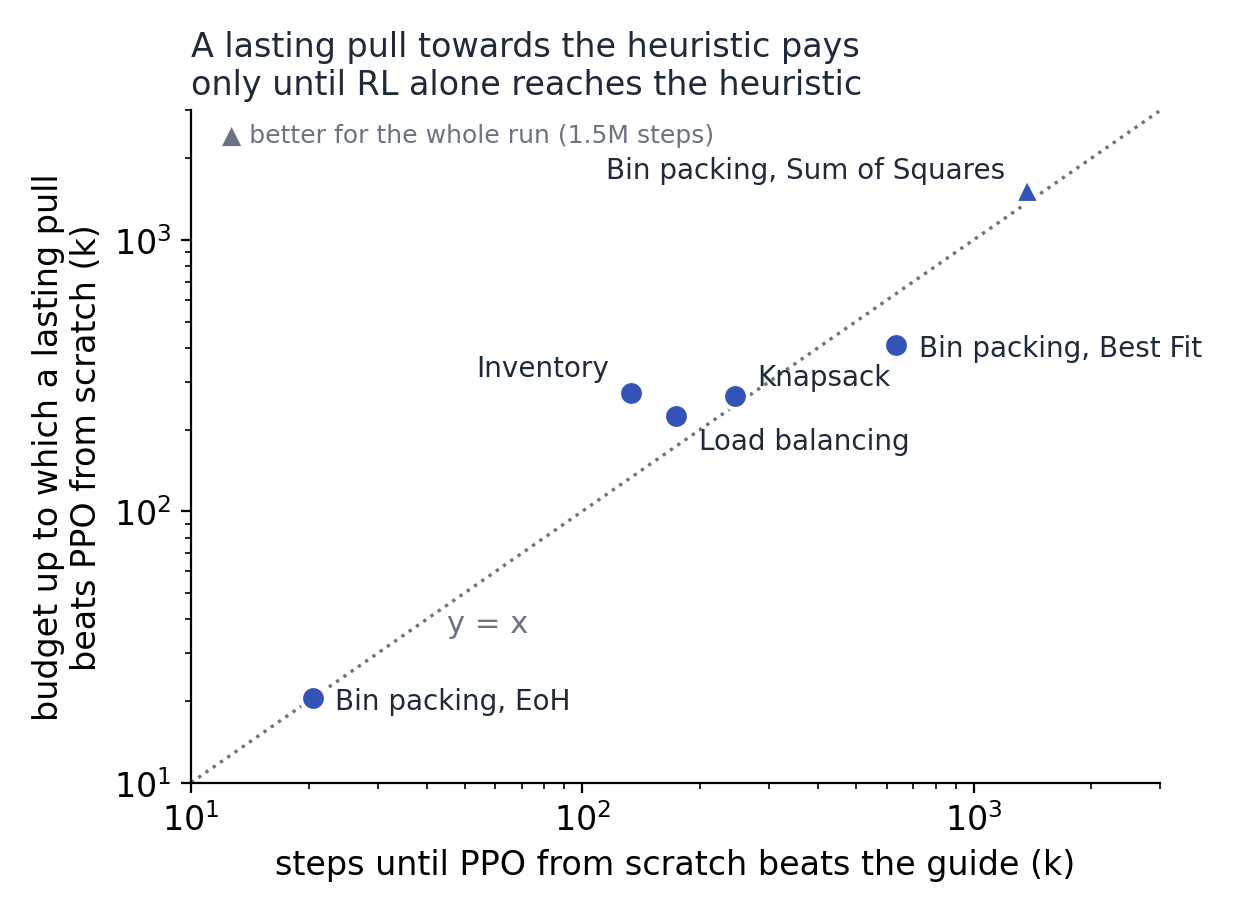
\includegraphics[width=0.6\linewidth]{regime.png}
\caption{Per experiment: the budget up to which the methods with a lasting pull (mean of five) beat PPO from scratch,
against the steps PPO from scratch needs to pass the guide (\texttt{report/regime.py}).}
\label{fig:regime}
\end{figure}

\paragraph{The Crafter study's methods on our problems.} The colleague's three arms, as in his \texttt{train.py}:
imitation from scratch (cross-entropy to $a_H$ on every visited state, coefficient 1 annealed to 0 by 25\%, or 0.1
held), and a residual prior $\beta\,\mathbf 1[a = a_H]$ added to the logits of networks that do not see $a_H$
($\beta = 2, 4, 8$; small initial actor, no critic warm-up). Annealed imitation is one of the best methods without a
simulator: better than PPO from scratch in four experiments, worse in one (load balancing), and, with DAgger $\to$ PPO, the best inventory result
(6.68), without a warm start. It is kickstarting with a faster schedule (25\%
instead of 50\%), which beats our kickstarting. Held imitation is as bad as our held anchor (better in 1, worse in
4). The residual prior reverses the Crafter ranking: $\beta = 2$ better in 1 and worse in 1, $\beta = 4$ 2 and 2,
$\beta = 8$ (the best on Crafter) 0 and 3. A stronger prior is a stronger lasting pull.

\paragraph{Making the held pull fade.} The same methods, with the pull decaying linearly to zero by 50\% of training:
\begin{itemize}[leftmargin=*]
\item \emph{Residual prior $\beta = 4 \to 0$}: mean rank 16.8 against 20.5 held (of 40 methods; PPO from scratch 23.3); the losses on load balancing and
  inventory disappear (1.63, 6.71, equal to PPO from scratch), but so do its wins (Sum of Squares, knapsack).
\item \emph{DQfD, demonstration share $0.5 \to 0$ and margin loss $\to 0$}: it leaves the heuristic (bin packing
  3.3--4.0\% instead of 9.7--11.6\%) and is the best off-policy result on knapsack (1.42\%, better than PPO from
  scratch), but it is worse on load balancing and inventory and far behind the PPO methods on bin packing.
\item \emph{IQL offline $\to$ online, demonstration share $0.5 \to 0$}: still stuck at the heuristic (0 better, 5
  worse). Its demonstrations are not what holds it: see the diagnosis below.
\item \emph{BC or IQL + HUBL $\to$ PPO + annealed imitation} (to 0 by 25\%, instead of the KL to the clone): about
  as good as the KL versions (better in 3 and 2 experiments, worse in 1), so the form of the fading pull matters
  little.
\end{itemize}

\paragraph{A pull that fades by itself: the Q-filter.} BC or IQL + HUBL warm start, 10 critic-only updates, then PPO
plus cross-entropy to $a_H$ with coefficient 1, applied only on the visited states where a critic
$Q(s,a)$ (regressed on the PPO returns of the actions taken) rates $a_H$ strictly above the policy's greedy action (Nair
et al., 2018). With $\ge$ instead of $>$ the filter fires wherever the policy already agrees with the heuristic and
locks it there. It does not work here: better than PPO from scratch only with Sum of Squares, worse in three
experiments (knapsack 2.2--2.5\%, load balancing 1.72, inventory 6.89--6.93, all near the guide), mean rank 28--29
of 40. The filter fires on only 1--4\% of states after the first updates, but those are the states where the policy
tries to depart from the heuristic, and an on-policy $Q$ is least accurate there, for actions the policy rarely takes.
Wherever it rates the heuristic's action higher, the departure is undone with full weight, so the policy stays close to
the heuristic. A Q-filter needs a critic that is reliable for the actions it compares, which on-policy PPO does not
provide.

\paragraph{A pull that ends when it is no longer needed: the performance gate.} Imitation (cross-entropy to $a_H$,
coefficient 1, from scratch or after BC or IQL + HUBL) stays on until the policy matches the heuristic; then it is
switched off for good. Every 10 iterations the greedy policy and the heuristic play the same 4 fresh training episodes
(never the evaluation episodes; these steps are counted in the budget), and the gate opens after the policy is at least
as good twice in a row. It opens after a median of 44--300k steps, before PPO from scratch passes the guide in five
experiments (with EoH, which PPO from scratch passes after 20k steps, it opens at 130--300k: cloning a weak heuristic
first costs time there). From scratch, \emph{performance-gated imitation} is better than PPO from scratch in two
experiments (Sum of Squares, EoH) and never worse, mean rank 12.2 of 40 (fourth, after the two Rollout-DAgger variants and online IQL with $\gamma = 0.99$;
the best of the PPO methods without a simulator), and better than kickstarting (16.2), the same loss on a fixed
schedule. After a warm start the gate adds nothing over the KL to the clone (BC 15.3, IQL + HUBL 15.0, against 13.5
and 12.5). The gate does what the fixed schedules
need tuning for: the pull lasts as long as the policy is below the heuristic, which is the regime in which a pull
helps.

\paragraph{A stronger teacher: rollout labels without the significance test.} Rollout-DAgger with the plain argmax
of the 32-sample estimates (no test before leaving the heuristic's action): better than PPO from scratch in five
experiments and never worse, the most of any method. Its labels are much better where the guide is weak: the
distilled teacher starts at 2.9\% waste with Best Fit (8.2\% with the test, 9.7\% Best Fit itself), and after PPO
it ends at \textbf{1.18 $\pm$ 0.09\%}, the best Best Fit result of all methods, with the smallest spread. Knapsack:
1.38\%, load balancing 1.59, both better than PPO from scratch. Where the guide is already near-optimal, the noisy
argmax costs: Sum of Squares 2.05\% (1.59 with the test), inventory 6.73 (6.69). Its mean rank (10.2) is below the
version with the test (6.8) for that reason. The test should be chosen by the guide's quality: off for a weak guide,
on for a strong one. Figure~\ref{fig:release} shows the learning curves of these variants.

\begin{figure}[p]
\centering
\begin{subfigure}{\linewidth}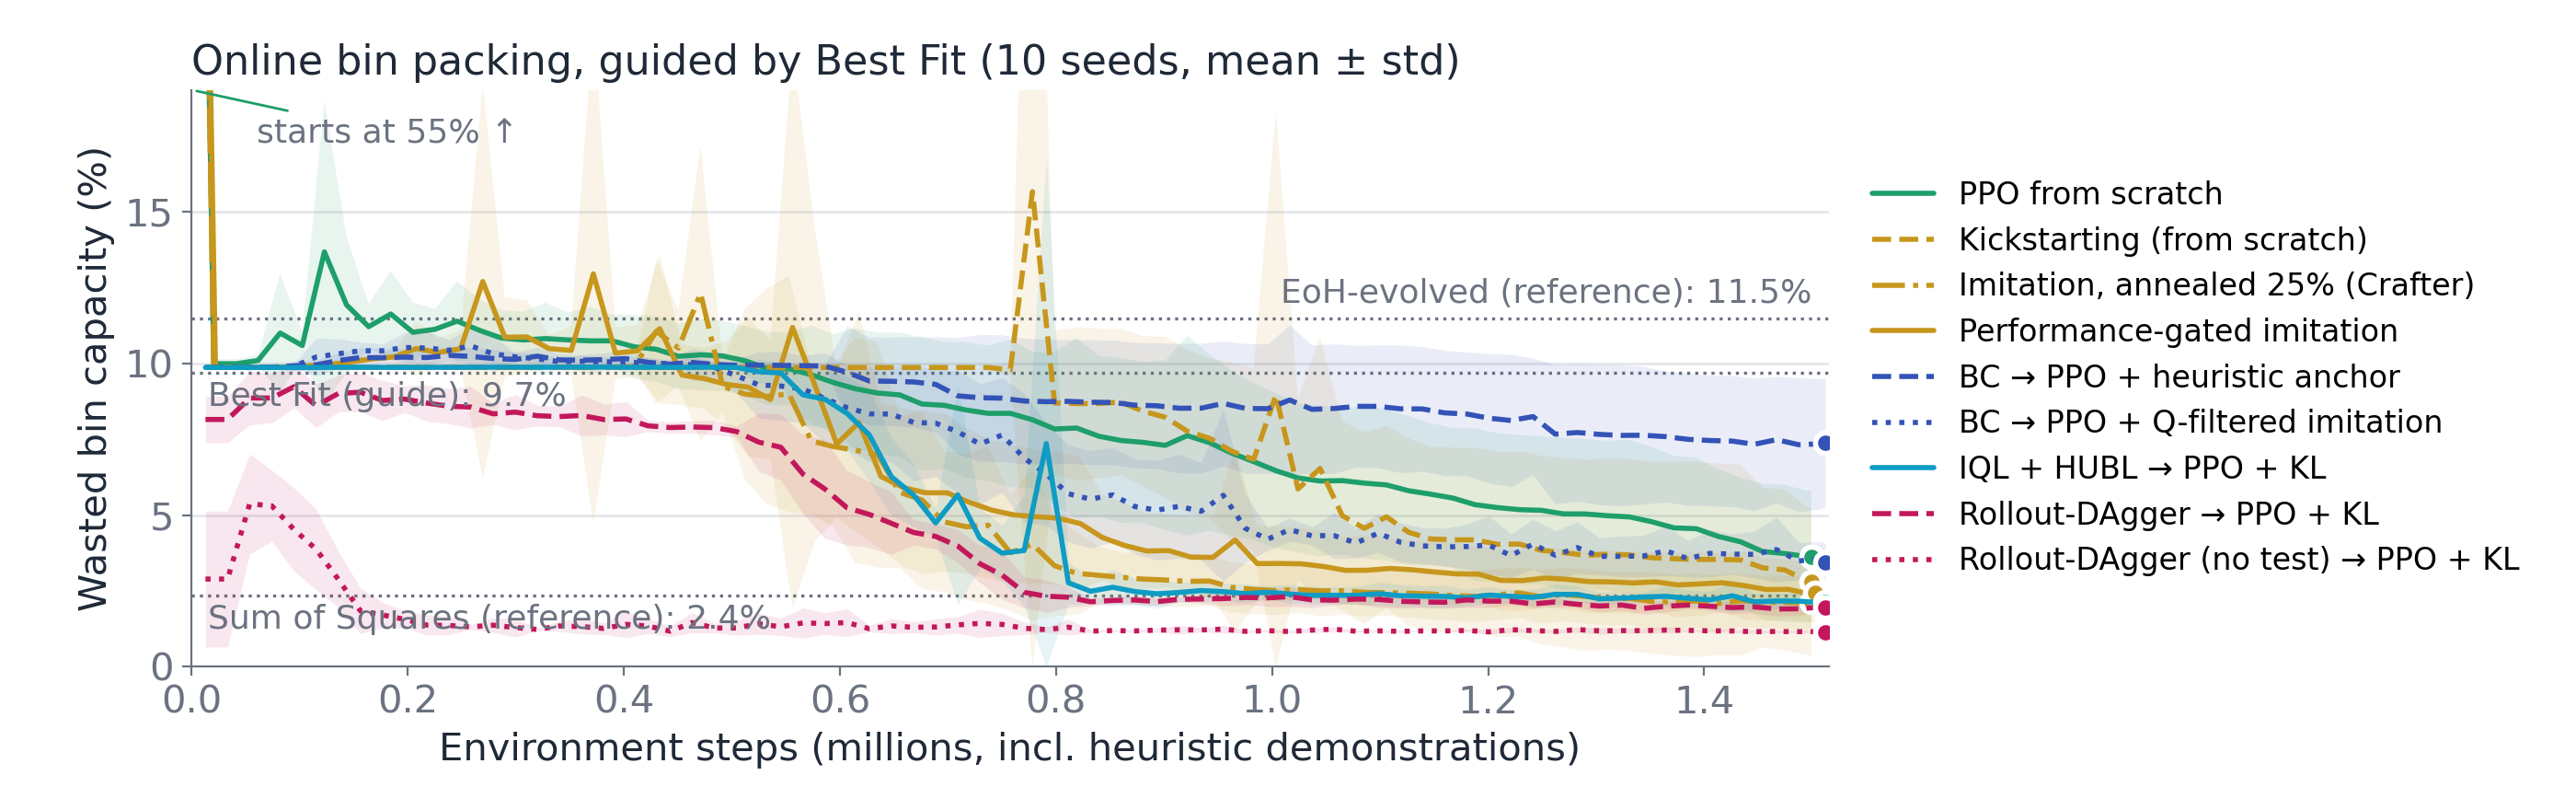
\includegraphics[width=\linewidth]{binpack_toy/best_fit/learning_curves_release.png}\end{subfigure}
\begin{subfigure}{\linewidth}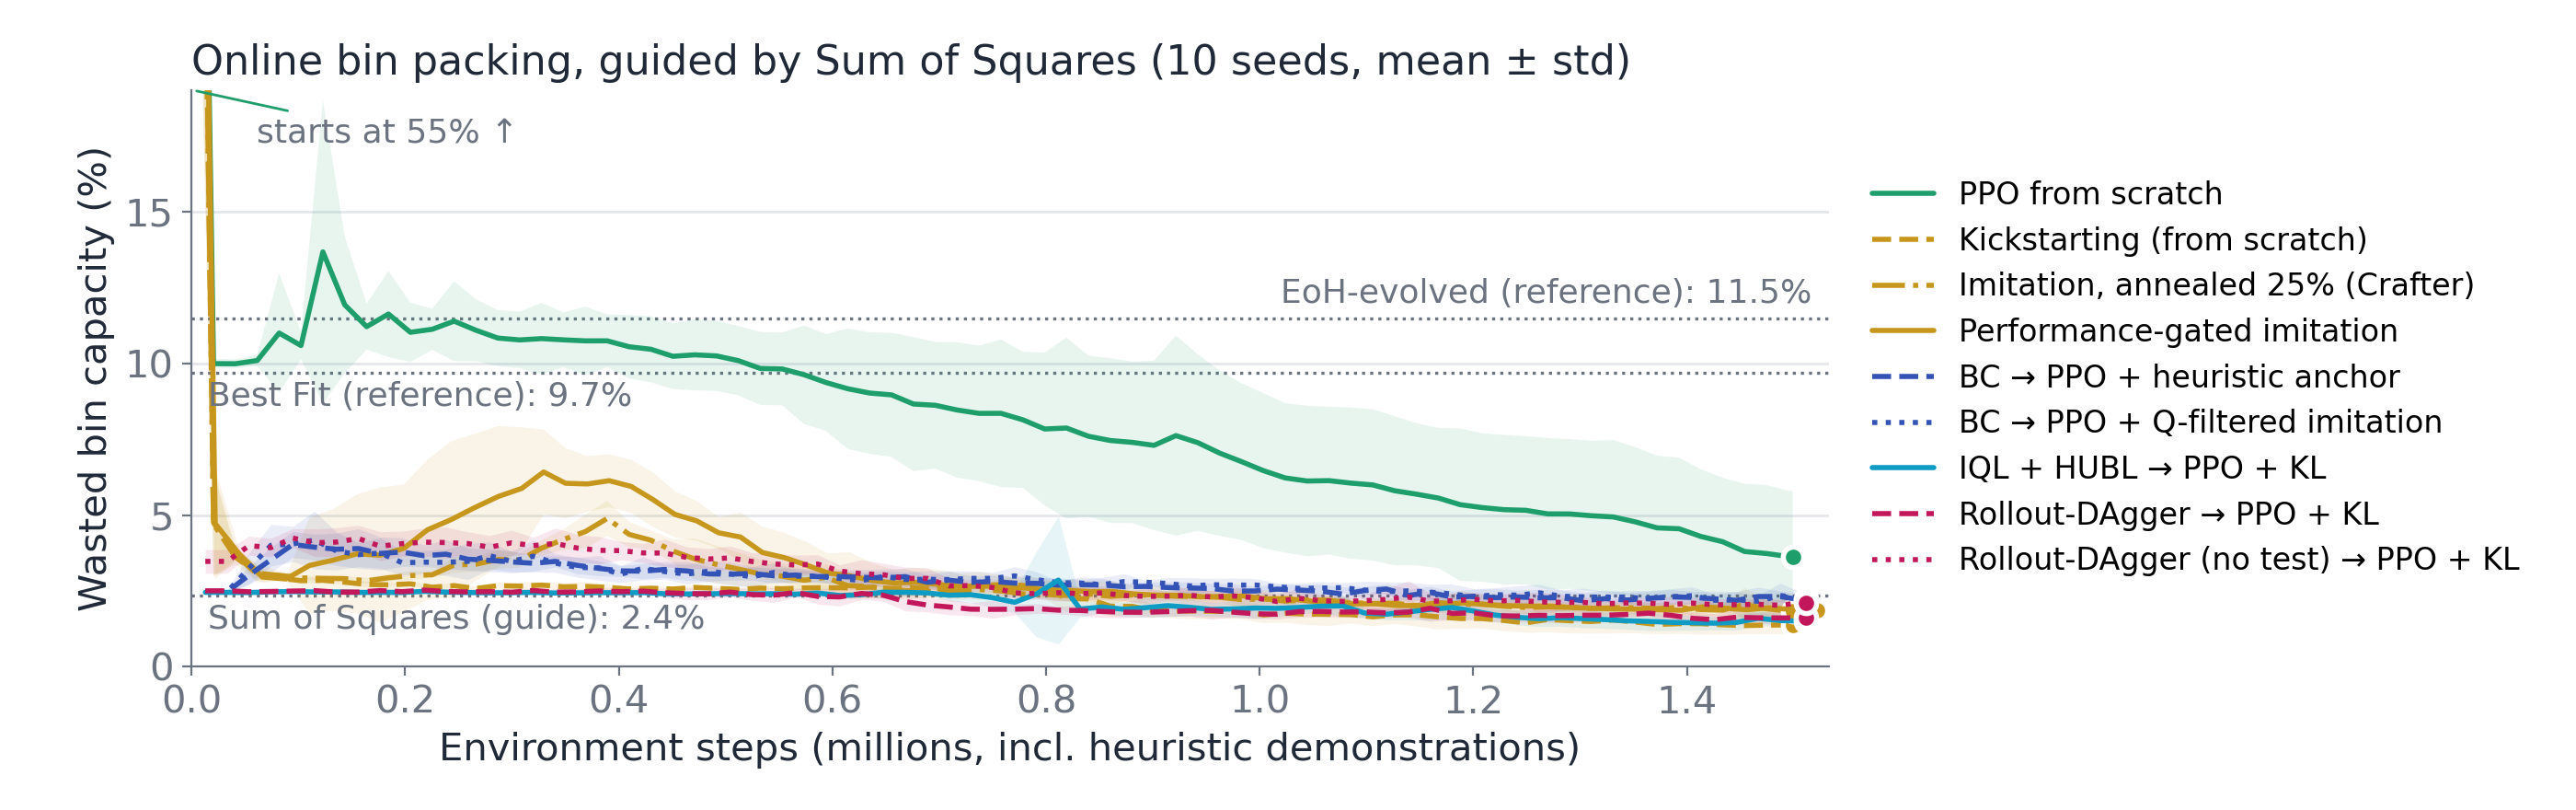
\includegraphics[width=\linewidth]{binpack_toy/sum_of_squares/learning_curves_release.png}\end{subfigure}
\begin{subfigure}{\linewidth}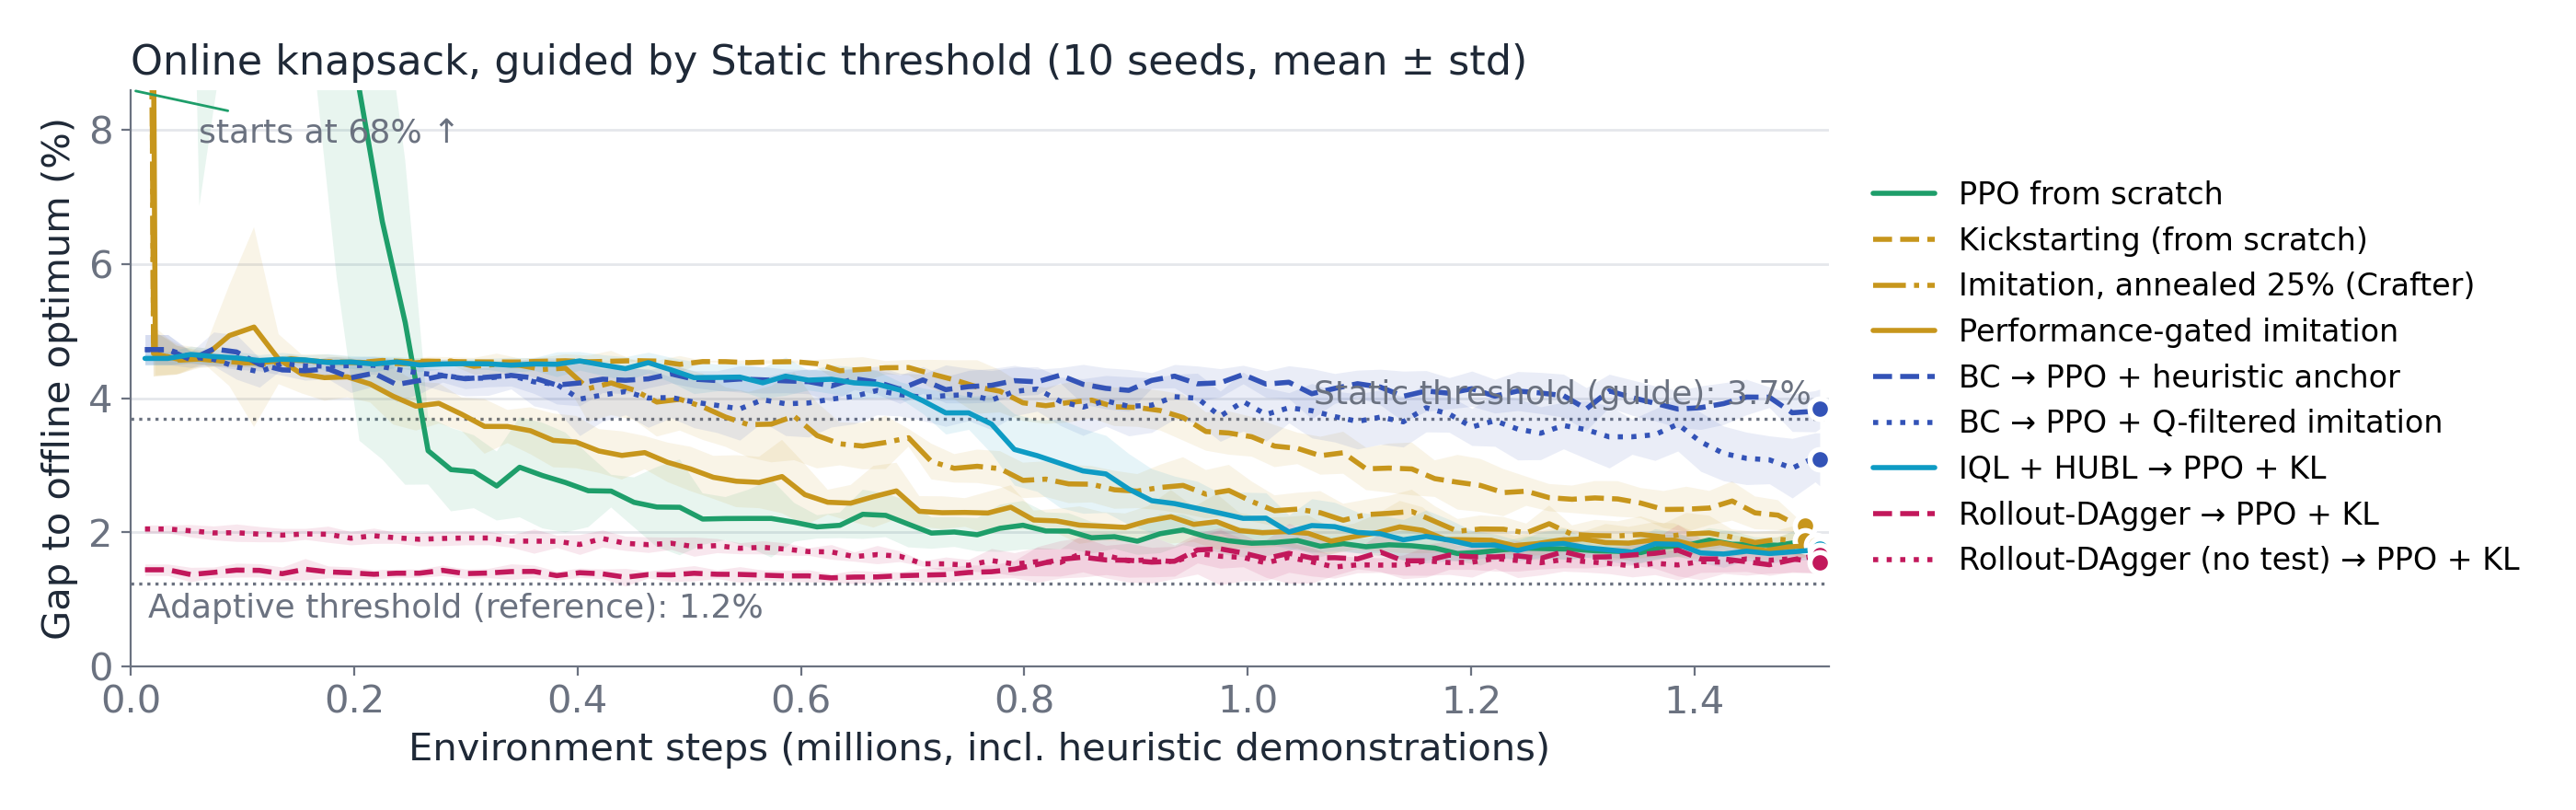
\includegraphics[width=\linewidth]{knapsack/static_threshold/learning_curves_release.png}\end{subfigure}
\begin{subfigure}{\linewidth}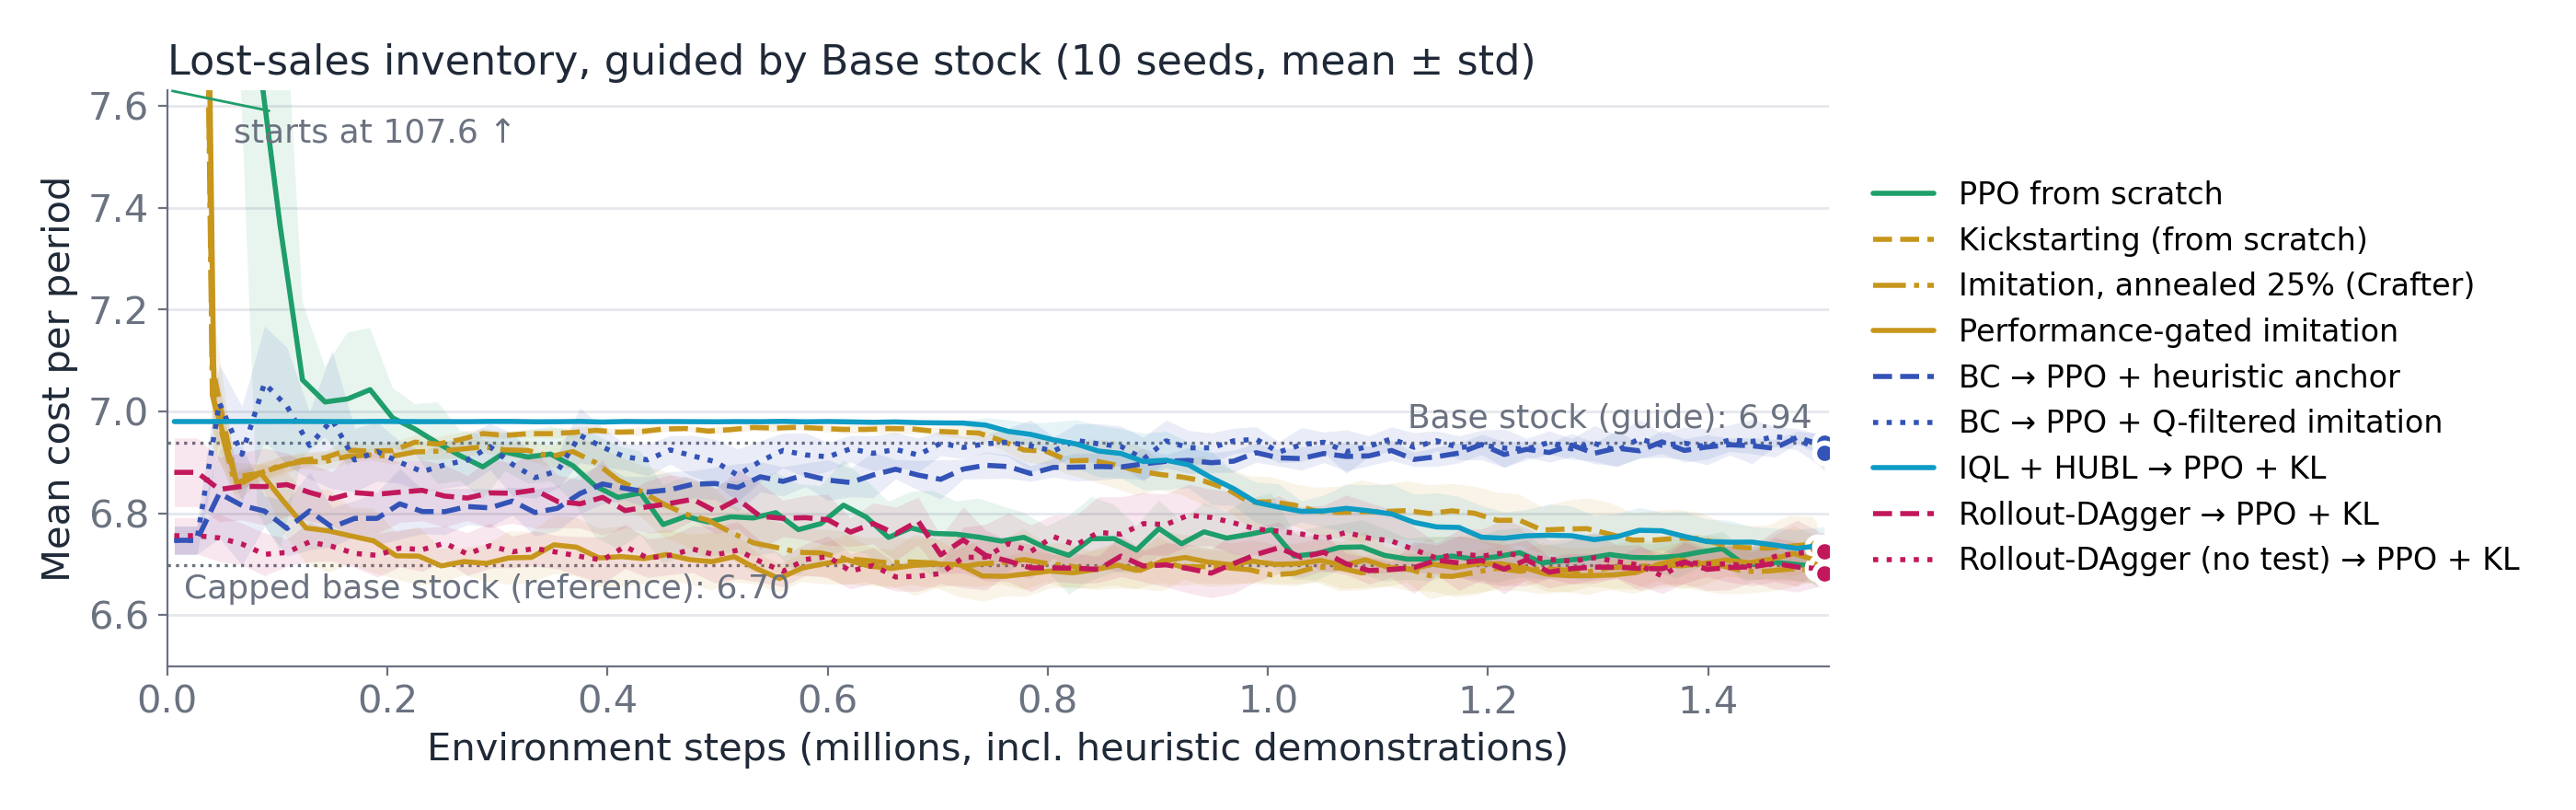
\includegraphics[width=\linewidth]{inventory/base_stock/learning_curves_release.png}\end{subfigure}
\caption{How the pull ends: a fixed schedule (kickstarting, annealed imitation, KL to an IQL + HUBL clone), never
(constant anchor), state by state (Q-filter), or when the policy matches the heuristic (performance gate); and the
rollout teacher with and without the significance test. Four of the six experiments; all six are in
\texttt{results/*/*/learning\_curves\_release.png}.}
\label{fig:release}
\end{figure}

\paragraph{Why online IQL never leaves the heuristic, and a fix.} With the heuristic's data faded out, IQL offline
$\to$ online still ends exactly at the guide (Best Fit: 9.86\% on the 64 curve episodes at every evaluation of a
300k-step diagnostic run). Its critic is not the problem: on the training batches it rates another action above the
stored one in 30--45\% of the states. The actor is. Advantage-weighted regression maximises
$\exp(\beta A)\log\pi(a|s)$; per-step advantages here are of order 0.01--0.1 (a placement changes the final bin
count only rarely), so with $\beta = 3$ every weight is $\approx 1$ and the update is behaviour cloning of the replay
buffer. Since the buffer is filled by the actor itself, starting from the heuristic, the actor clones itself and
stays at the heuristic: a lasting pull that no fading of the demonstrations removes. $\beta = 10$ is not a way out (it
collapsed the actor on knapsack). The fix is to make the temperature scale-free: \textbf{normalise the advantages by
their standard deviation in each batch}, $w = \min(\exp(\beta A/\sigma_A), 100)$, $\beta = 3$, with the fading
demonstration share. This one change turns the worst method into one of the best:
\begin{itemize}[leftmargin=*]
\item knapsack 1.25 $\pm$ 0.07\% (PPO from scratch 1.67, the best previous method 1.30, the adaptive-threshold
  reference 1.24); load balancing 1.58 $\pm$ 0.01 (1.64; best previous 1.59); inventory 6.66 $\pm$ 0.02 (6.71; best
  previous 6.68, capped base stock 6.70). All three significantly better than PPO from scratch, the best of all methods
  on knapsack and inventory, and on load balancing second only to its $\gamma = 0.99$ version below.
\item On bin packing it learns fastest of all but does not keep it: with Best Fit every seed reaches 1.19\%
  waste (on the 64 curve episodes) within 33--115k steps and is still there at 300k, as good as the best final result of
  any method; then it degrades, to 3.1\% at 750k and at the end (3.11 $\pm$ 1.04\%, no better than PPO from scratch).
  The same with Sum of Squares (1.44\% at 300k, 2.80\% at the end) and EoH (1.32\% at 300k, 3.30\% at the end);
  see Figure~\ref{fig:fade}.
\end{itemize}
\begin{itemize}[leftmargin=*,resume]
\item The late decline on bin packing is not caused by the fading demonstrations: with the heuristic's data held at
  half of every batch (\emph{normalised AWR, held}), Best Fit still ends at 3.95 $\pm$ 0.89\%. The held version is
  instead the regime rule once more: it is, after the $\gamma = 0.99$ version below, the best method with the near-optimal Sum of Squares guide
  (1.33 $\pm$ 0.24\%, against 1.43 for kickstarting, the best before), which PPO from scratch needs 1.37M steps to
  pass, and much worse where PPO passes the guide early (knapsack 4.10\%, load balancing 1.66, inventory 6.88).
\end{itemize}
\begin{itemize}[leftmargin=*,resume]
\item The decline comes from the undiscounted bootstrap. With $\gamma = 0.99$ instead of 1 (fading, normalised; the
  last experiment we ran), bin packing keeps most of its fast start: Sum of Squares \textbf{1.15 $\pm$ 0.09\%}, the
  best result in that column (1.18\% at 300k, still 1.09\% on the curve episodes at the end), EoH 1.42 $\pm$ 0.20\%,
  Best Fit 2.11 $\pm$ 1.65\% (eight seeds at 1.0--1.9\%, two at 4.7 and 6.0\%). Load balancing improves to
  \textbf{1.57 $\pm$ 0.01}, the best in that column, inventory stays at 6.67. Knapsack, however, collapses (13.8\%):
  its capacity constraint couples the first and last of 200 decisions, and a discount of 0.99 (horizon $\approx$ 100)
  makes accepting early items look free. Mean rank 9.5 of 40, second only to Rollout-DAgger $\to$ PPO + KL, with no
  simulator; better than PPO from scratch in four experiments, worse in one (knapsack).
\end{itemize}
The discount is therefore a per-problem choice: $\gamma = 1$ where decisions are coupled over the whole episode
(knapsack), $\gamma < 1$ where the bootstrap over 200 steps destabilises the critic (bin packing). Choosing it by a
held-out validation run, or keeping the best checkpoint, are the obvious next steps.

\begin{figure}[t]
\centering
\begin{subfigure}{\linewidth}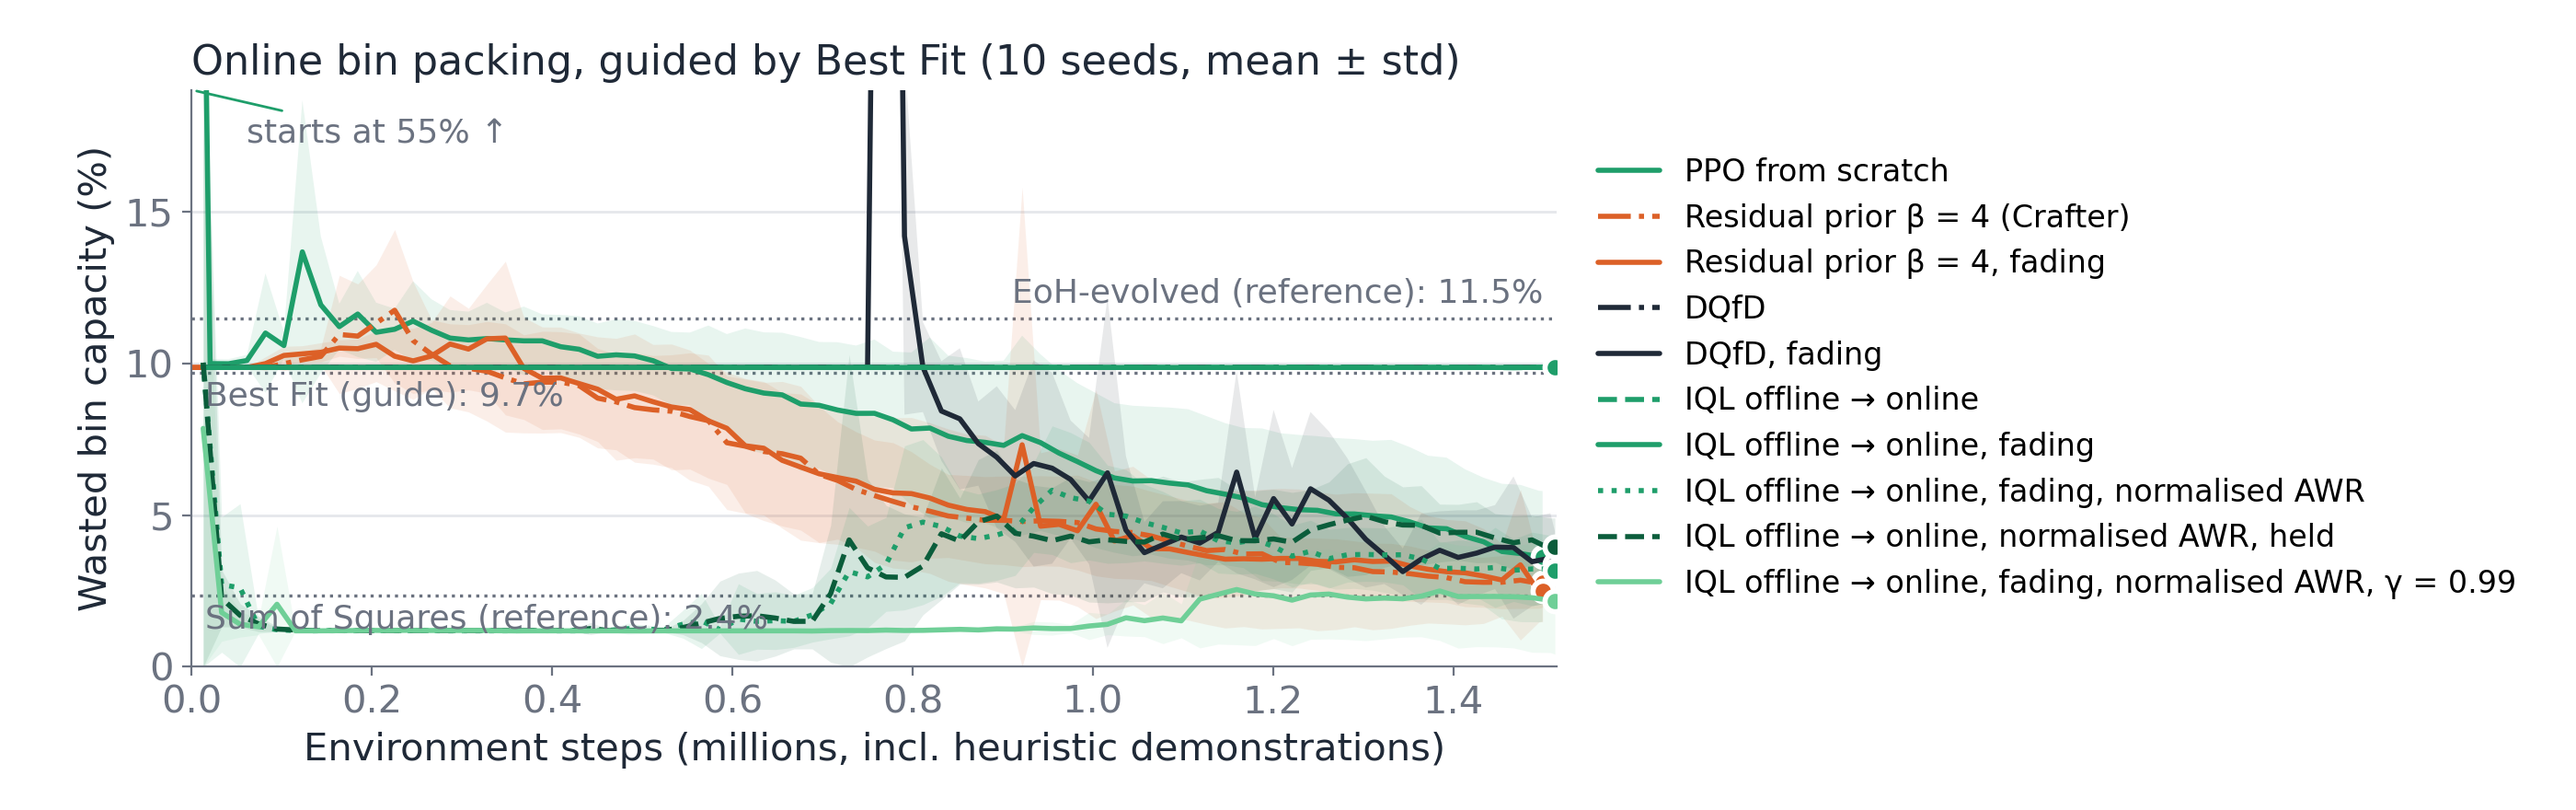
\includegraphics[width=\linewidth]{binpack_toy/best_fit/learning_curves_fade.png}\end{subfigure}
\begin{subfigure}{\linewidth}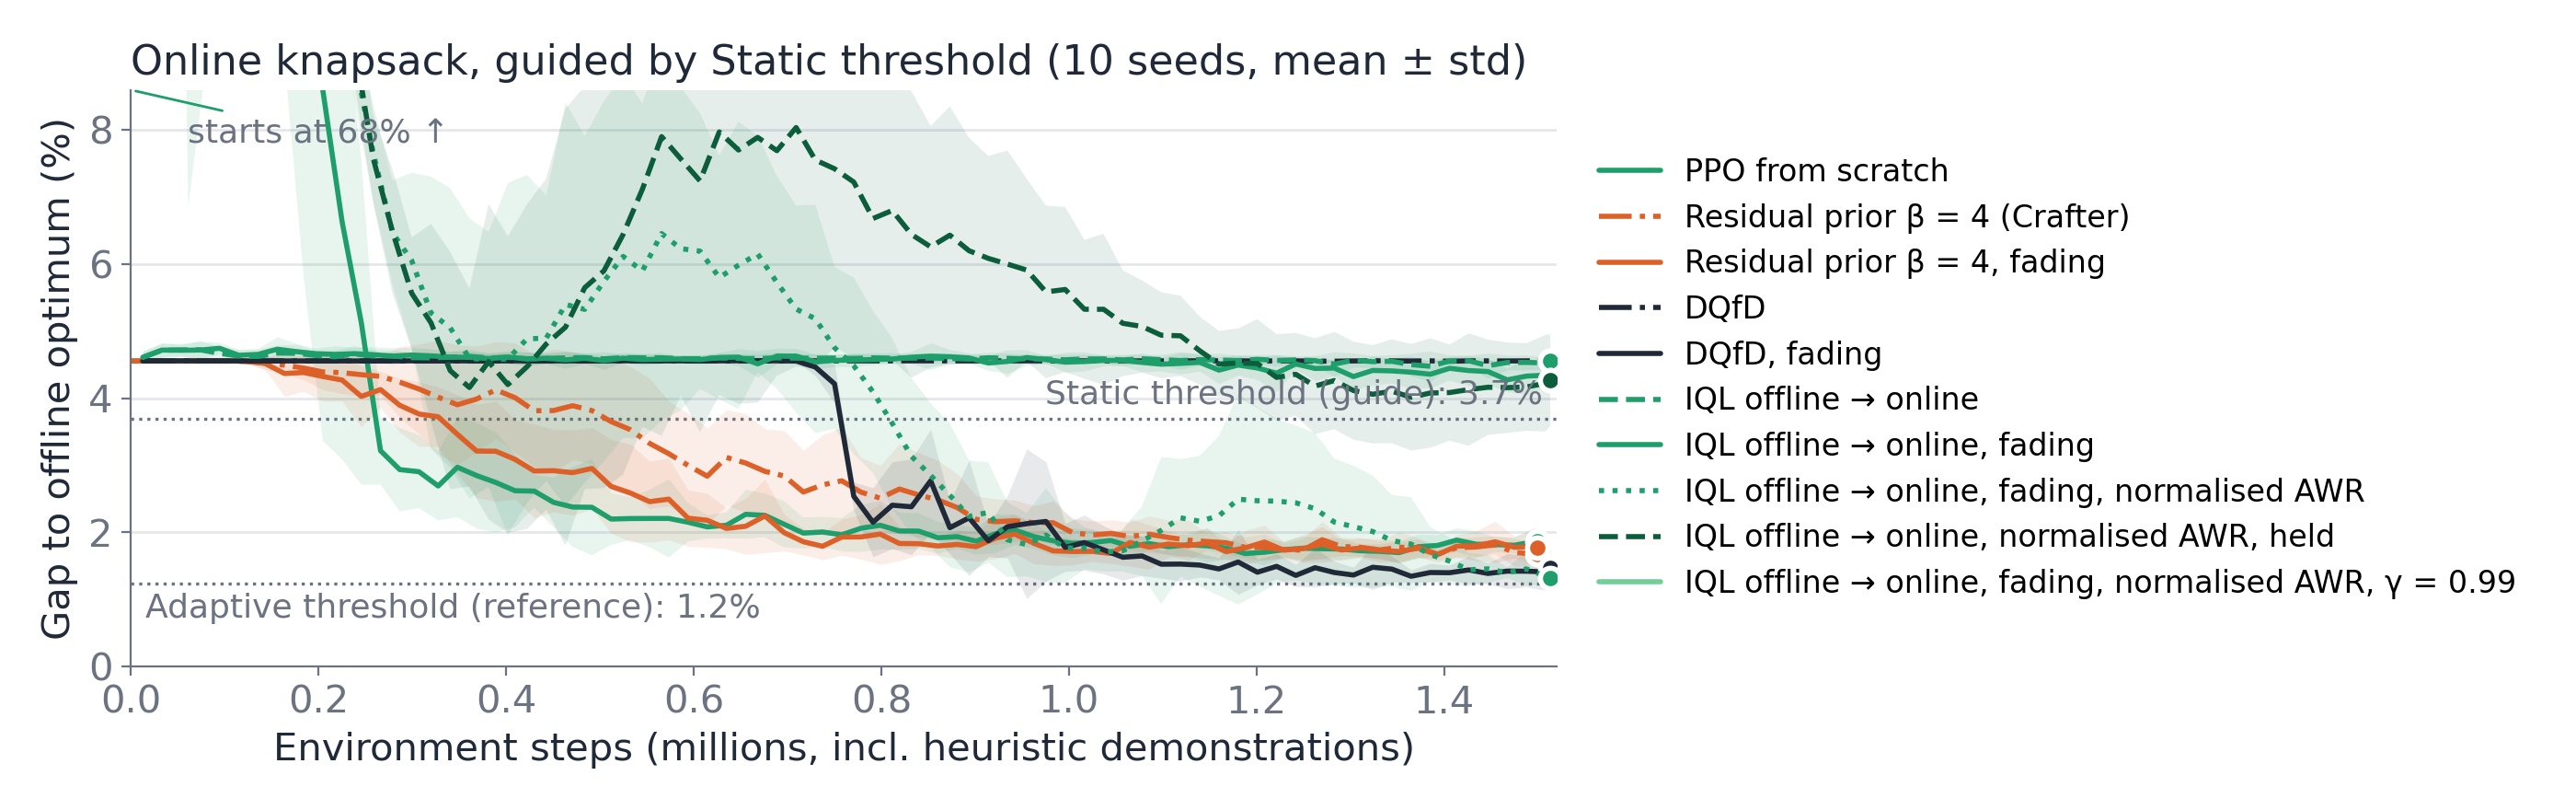
\includegraphics[width=\linewidth]{knapsack/static_threshold/learning_curves_fade.png}\end{subfigure}
\caption{The methods that hold the pull, their fading versions, and online IQL with normalised advantage weights
(fading, held, and $\gamma = 0.99$). Bin packing with Best Fit (top) and knapsack (bottom).}
\label{fig:fade}
\end{figure}

%FOLLOWUP-MORE

\section{Our methods on Crafter}
\label{sec:crafter}

To check that the regime, not the method, decides the ranking, we ran our offline methods in the colleague's Crafter
setup (\texttt{RL-AHD-Crafter/train\_ours.py}): his environment, heuristic, Nature-CNN PPO and scoring, unchanged.
Our arms: BC, DAgger, IQL and IQL + HUBL $\to$ PPO + KL, HuRL, BC $\to$ HuRL and Jump-Start RL, with 16,384 steps of
the heuristic (about 1.6\% of the budget, counted against it) and 10 critic-only updates; BC and DAgger learn only from
the heuristic's goal steps, where it is not exploring at random. Rollout-DAgger is left out: copying the environment
would reveal the pre-generated map, which the agent never sees. 3 seeds $\times$ 1M steps; Crafter score (geometric
mean of the 22 achievement success rates) over all training episodes and over the last 10\% of the steps.

\begin{table}[h]
\centering\small
\begin{tabular}{lcc}
\toprule
Method & score, all episodes & score, last 10\% \\
\midrule
\emph{heuristic alone} & \multicolumn{2}{c}{25.95} \\
plain PPO (his) & 7.53 & 10.22 \\
imitation, annealed by 25\% (his) & 10.63 & 14.07 \\
residual prior $\beta = 4$ (his) & 28.33 & 29.76 \\
residual prior $\beta = 8$ (his) & \textbf{28.71} & \textbf{30.88} \\
BC $\to$ PPO + KL & 9.05 & 11.05 \\
DAgger $\to$ PPO + KL & 7.54 & 9.43 \\
IQL $\to$ PPO + KL & 13.52 & 16.75 \\
IQL + HUBL $\to$ PPO + KL & 12.48 & 15.54 \\
HuRL & 7.50 & 9.21 \\
BC $\to$ HuRL & 8.17 & 9.73 \\
Jump-Start RL & 15.22 & 5.22 \\
\bottomrule
\end{tabular}
\caption{Crafter, 1M steps, mean of 3 seeds (seeds differ by at most 2.4 points; per-seed values in
\texttt{RL-AHD-Crafter/results/cross.csv}). His arms reproduce his own numbers (plain 7.76, imitation 11.27, residual $\beta = 8$ 27.97).}
\label{tab:crafter}
\end{table}

\begin{figure}[h]
\centering
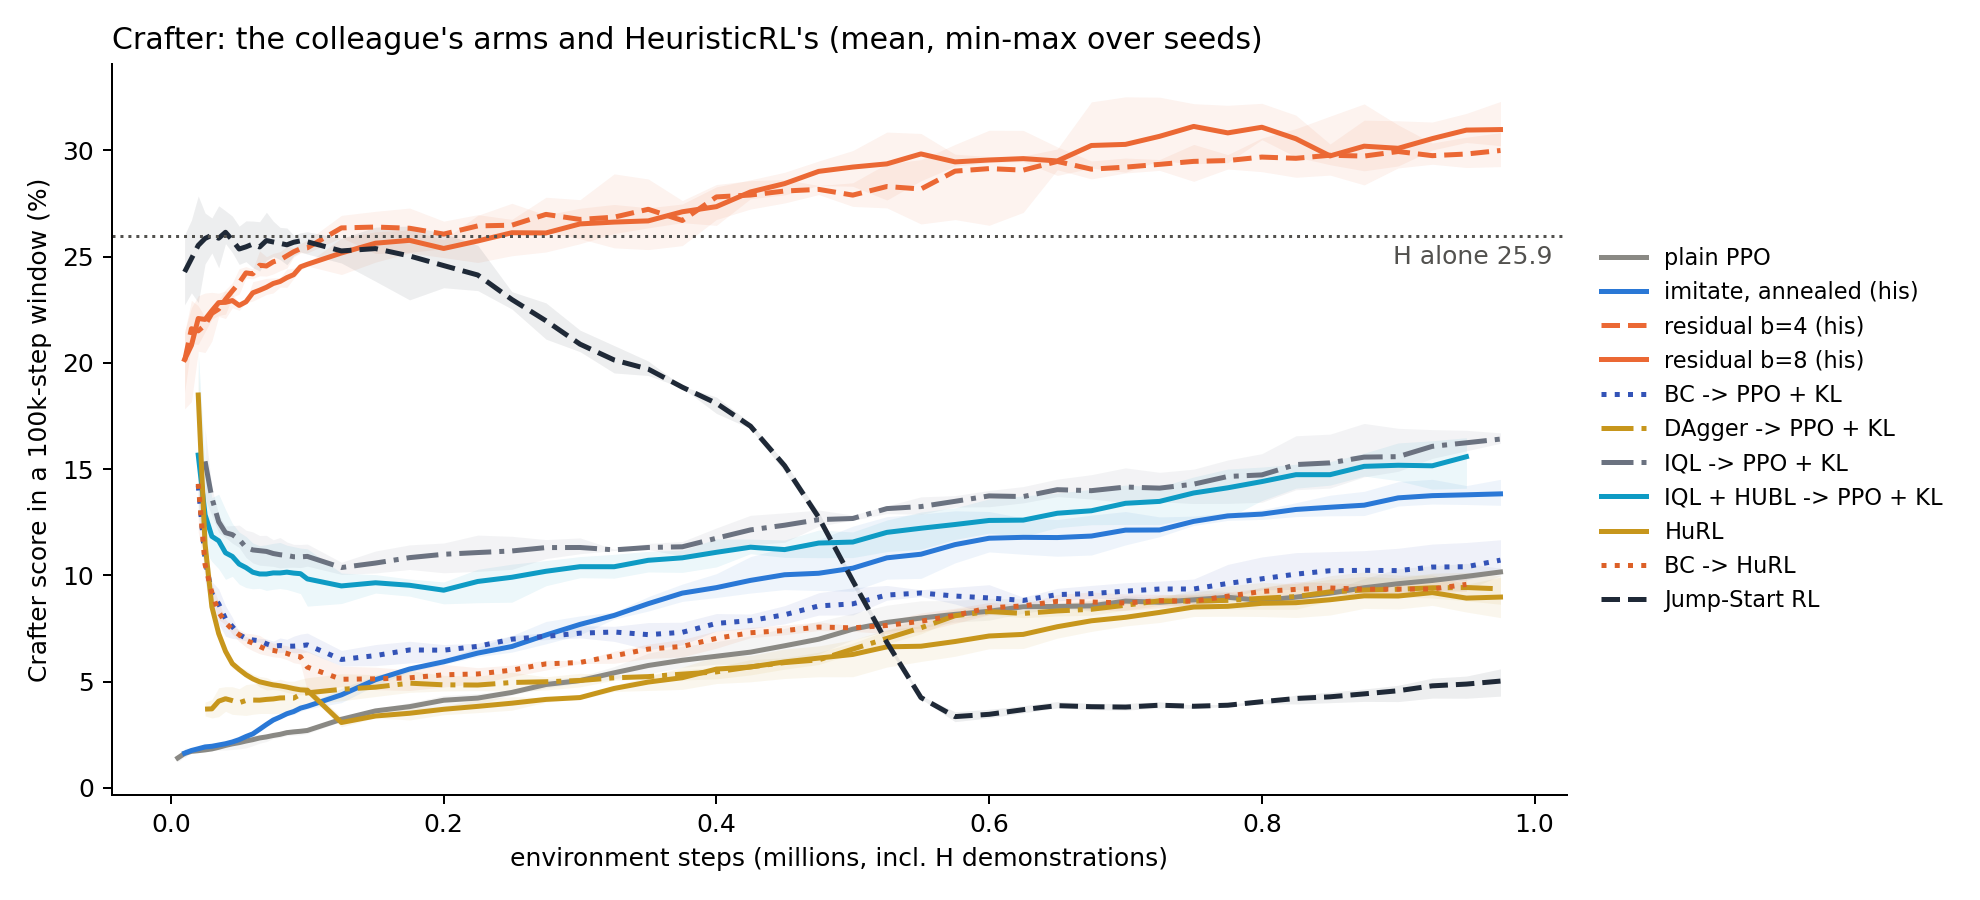
\includegraphics[width=\linewidth]{crafter_cross.png}
\caption{Crafter score in 100k-step windows (mean and min--max over 3 seeds). The heuristic's demonstration steps are
on the x-axis but not in the score.}
\label{fig:crafter}
\end{figure}

\begin{itemize}[leftmargin=*]
\item \textbf{The residual prior wins by far} (28.7 / 30.9, above the heuristic), as in his study. Here PPO alone is
  at a third of the heuristic after 1M steps, so a lasting pull is what pays (Figure~\ref{fig:regime}).
\item \textbf{Of ours, IQL $\to$ PPO + KL is best} (13.5 / 16.8), better than his annealed imitation (10.6 / 14.1) and
  plain PPO; IQL + HUBL is close. As on our problems, the IQL warm starts beat the BC and DAgger ones.
\item \textbf{The clones collapse.} The BC and IQL warm starts begin at 14--16 (below the heuristic, which uses
  hidden information: its exploration state and the decoded map) and drop within about 50k steps, even with the KL to
  the clone: BC to 6, the IQL clones to 10, from where they climb. The DAgger clone starts at only 4, possibly
  because on the states its own policy visits the heuristic's labels depend on its hidden exploration state. This is the collapse of RL-AHD-OBP and PIRLNav, and on a
  pixel CNN with a shared trunk ten critic-only updates do not prevent it.
\item \textbf{Jump-Start RL} is at the heuristic's level while the heuristic plays most of each episode (which is
  why its all-episodes score is high) and collapses to 5 when the prefix ends, worse than plain PPO: the policy never
  learned the early part of the game.
\item HuRL, with or without BC, and DAgger do not beat plain PPO.
\end{itemize}
So the two projects agree once the regime is taken into account: when RL alone is far below the heuristic within the
budget, keep the heuristic in the policy (residual prior); when RL alone can pass it, start from it and let it go.

\paragraph{Consistency across seeds.} Much of what the warm starts buy is a smaller spread. Standard deviation of the
final metric over 10 seeds, relative to PPO from scratch, averaged over the offline warm starts with a KL to the clone
(BC, DAgger, IQL, IQL + HUBL): 0.22 (Best Fit), 0.07 (Sum of Squares), 0.13 (EoH), 0.66 (knapsack), 0.81 (load
balancing), 1.00 (inventory). On bin packing a single run of PPO from scratch can end anywhere between about 1.8\% and
6\%; a warm-started run is close to its method's mean.

\paragraph{Related work on letting go of a prior policy.} Three lines of work address the same problem.
PIRLNav (Ramrakhya et al., 2023) fine-tunes a behaviour-cloned navigation policy with RL and finds that it collapses
unless the critic is trained alone first and the actor's learning rate is ramped up slowly, the same failure as our
naive BC $\to$ PPO and the same fix as our critic-only updates. Policy Expansion (PEX, Zhang et al., 2023) keeps the
offline (IQL) policy frozen in a policy set next to a new one and picks between their actions by the learned $Q$,
so the prior is used only where $Q$ prefers it. The Q-filter of Nair et al.\ (2018) applies an imitation loss only on
states where the critic rates the demonstrated action above the policy's own. The last two are ways of letting the
pull fade state by state rather than on a fixed schedule; we test the Q-filter, and a performance gate that ends the
pull once the policy matches the heuristic, below.

\section{Conclusions}

\begin{itemize}[leftmargin=*]
\item \textbf{The regime decides.} A pull towards the heuristic that lasts the whole run helps only while RL alone is
  below the heuristic: on our problems the budget up to which it beats PPO from scratch tracks the steps PPO from
  scratch needs to pass the guide (Figure~\ref{fig:regime}). Where PPO alone stays far below the heuristic for the
  whole budget (Crafter, RL-AHD-OBP) the lasting pull is the best method; where it can pass the heuristic (five of
  our six experiments) every lasting pull ends at or near the heuristic. The same methods, run in both settings,
  reverse their ranking (residual prior $\beta = 8$: best on Crafter, among the worst here).
\item \textbf{The most reliable way to improve on the heuristic here} is to improve the heuristic first and let RL
  finish: Rollout-DAgger $\to$ PPO + KL has the best mean rank, is significantly better than PPO from scratch in four
  of six experiments and never worse, and is faster and better than the guide in all six. Without the significance
  test its labels are stronger for weak guides (Best Fit: 1.18\%, the best in that column, better than PPO from
  scratch in five experiments) and noisier for strong ones. It needs a simulator that can redraw the unrevealed future
  and 80--500M simulated steps per run.
\item \textbf{Without a simulator}, IQL (+ HUBL) $\to$ PPO + KL from 64 heuristic episodes, or, without any warm
  start, imitation of the heuristic that ends on a schedule (annealed by 25\%, from the Crafter study) or when the
  policy matches the heuristic (performance gate; never worse than PPO from scratch). IQL $\to$ PPO + KL is also our
  best method on Crafter.
\item \textbf{Off-policy RL with the heuristic's data can be the best method}, but only once nothing in it holds the
  policy at the heuristic. Online IQL's advantage-weighted actor silently reduced to cloning its own buffer; with
  advantages normalised per batch it is the best method on knapsack and inventory, and the fastest on
  bin packing, where it then degrades unless the discount is below 1 ($\gamma = 0.99$: best on Sum of Squares and load
  balancing, second-best mean rank of all, but knapsack then fails). No simulator needed.
\item \textbf{When the pull should end is better decided by performance than by a critic.} The performance gate
  releases the pull before PPO from scratch would pass the guide in five of six experiments and needs no schedule;
  the Q-filter, which ends it state by state where an on-policy critic prefers the policy's action, keeps the policy
  near the heuristic.
\item \textbf{Most of the value is consistency and speed.} On bin packing the warm starts remove most of PPO's seed
  variance (standard deviation 7--22\% of PPO from scratch); elsewhere they reach the guide 10--20 times sooner. The
  final level is set mostly by the problem, not the guide: the weak EoH guide led to one of the best bin-packing
  results.
\item \textbf{A transferred LLM-evolved heuristic} is a weak guide on a different item distribution (worse than Best
  Fit), but every method that lets it go ends far below it.
\end{itemize}

\paragraph{Relation to the companion projects.} RL-AHD-OBP distils the same EoH heuristic into a convolutional PPO
policy for Weibull bin packing (capacity 100): there, cloning reaches the teacher, naive PPO destroys the clone, and
only PPO anchored to the teacher at a constant 0.1 with a 4$\times$ batch beats it. A colleague's Crafter project
compares plain PPO, kickstarting-style imitation (annealed and constant) and a residual policy with prior strength
$\beta = 2$--8 on goal steps only; the residual policy beats both PPO and the heuristic (34.4 vs 19.2 and 26.0 at 5M
steps). We ran his methods on our problems (Section~\ref{sec:followup}) and ours on Crafter
(Section~\ref{sec:crafter}); a detailed comparison of the two set-ups is in \texttt{docs/comparison\_crafter.md}.
Both companion projects are in the regime where the heuristic is far beyond PPO's reach within budget, the opposite of
most of ours, which explains why their best methods (a lasting anchor, a strong residual prior) are among our weakest.

\paragraph{Limitations.} 10 seeds and one training budget (Crafter: 3 seeds, 1M steps); method-specific hyperparameters untuned (e.g.\ the
residual prior $\kappa = 3$, below the colleague's best $\beta$ of 4--8; the demonstration share and margin of the
off-policy methods; the significance level of the rollout labels); small problems whose guides are fully observable
functions of the state, so cloning is almost exact. Rollout-DAgger's simulated steps are not counted in its budget.
Q2 uses the first evaluation below the guide on 64 episodes, which is noisy for methods that start at the guide's
level; it also takes the median over the seeds that pass the guide at all.

\paragraph{Reproducing.}
\begin{itemize}[leftmargin=*]
\item \texttt{python run\_experiments.py --problem P [--demo H] --seeds 10} trains all methods for one experiment,
  with \texttt{P} one of \texttt{binpack}, \texttt{knapsack}, \texttt{load\_balancing}, \texttt{inventory} and, for
  bin packing, \texttt{H} one of \texttt{best\_fit}, \texttt{sum\_of\_squares}, \texttt{eoh\_evolved};
  \texttt{--variants} and \texttt{--reuse} train a subset and keep the rest;
\item \texttt{python rollout\_reference.py} evaluates the guides and their rollout improvements;
\item \texttt{python plot\_results.py} redraws every figure; \texttt{python report/make\_tables.py} regenerates the
  tables of this report.
\item \texttt{python report/regime.py} draws Figure~\ref{fig:regime};
\item Crafter: in \texttt{RL-AHD-Crafter}, \texttt{bash run\_cross.sh} trains the cross-test arms (3 seeds, 1M steps,
  GPU) and \texttt{python plot\_cross.py --runs runs\_cross} scores them and draws Figure~\ref{fig:crafter}.
\end{itemize}

\end{document}
